%% Things to be optionally fixed:
%% *  fix that f is used as frequency (replace with omega) and also as arbitrary function f(t) 
%% *  get rid of the term "response function" for susceptibility
%% *  ensure more consistent usage of "dispersion curve", "dispersion relation" and "solution of Maxwell equations"

\section{Electrodynamics of local homogeneous media} 
\subsection{Electromagnetic wave in vacuum}
\paragraph{Maxwell equations}  %{{{
In the realm of classical physics, the electromagnetic phenomena are governed by the \textit{Maxwell equations} in the following form.
We assume here that no free charges and no sources of currents are present: 
\begin{equation} \nabla \cdot  \D = 0, \label{eq_me1}\end{equation}  
\begin{equation} \nabla \cdot  \B = 0, \label{eq_me2}\end{equation}  
\begin{equation} \nabla \times \E = -\frac{\partial \B} {\partial t}, \label{eq_me3}\end{equation}  
\begin{equation} \nabla \times \HH =  \frac{\partial \D} {\partial t}, \label{eq_me4}\end{equation}  
where $\E$ and $\HH$ are the electric and magnetic vector fields, and $\D$ and $\B$ are the electric and magnetic displacements,
 respectively. These two pairs of field and displacement are related in a similar way as a force is related to the deformation. % note that Simovski2007 regards the current J as force, and E as the deformation!
 The \textit{constitutive relations} depend on the properties of the medium the wave propagates in, and in vacuum they take the simplest possible form:
\begin{equation}		\D = \varepsilon_0	\E, \quad\quad\quad						\B = \mu_0			\HH,				 \label{eq_ce}\end{equation}
$\varepsilon_0 \approx 8.85\cdot10^{-12}$ F/m being the \textit{vacuum permittivity} and $\mu_0 = 4\pi \cdot 10^{-7} \approx 1.25\cdot10^{-6}$ H/m he \textit{vacuum permeability}. 
Pages \pageref{starttext}--\pageref{endtext} of this thesis will be concerned with computation, interpretation, and experimental verification of the solutions of Eq. (\ref{eq_me1}--\ref{eq_me4})  for specific choices of constitutive relations.
%}}}
\paragraph{Wave equation in vacuum} %{{{
The pair of first-order differential equations (\ref{eq_me3}, \ref{eq_me4}) can be converted to a single second-order differential equation. To this end, we apply an extra curl operator $\nabla\times$ from the left, and substituting one equation into the another, we obtain two curl operators on the left hand side and two derivatives on the right hand side: 
\label{starttext}
\begin{equation} \nabla\times (\nabla\times \E) = \nabla\times \left(- \frac{\partial \B} {\partial t}\right) = -\mu_0 \frac{\partial}{\partial t} \left(\nabla\times \HH\right) 
= -\mu_0 \frac{\partial^{2} \D}{\partial t^{2}} = -\mu_0 \varepsilon_0 \frac{\partial^{2} \E}{\partial t^{2}}.  \label{eq_elim}\end{equation}
Using the vector calculus identity
\begin{equation} \nabla\times (\nabla\times \E) \equiv \nabla (\nabla \cdot \E) - \nabla^2 \E, \label{eq_rotrot}\end{equation}
we obtain the \textit{wave equation} for the electric field in vacuum: 
\begin{equation}  \nabla (\nabla \cdot \E) - \nabla^2 \E = -\mu_0 \varepsilon_0 \frac{\partial^{2} \E}{\partial t^{2}}.  \label{eq_wave}\end{equation}
%Note this holds for each component of electric field independently. -- NOT: the divergence is not independent of other components
Starting with Eq. (\ref{eq_me4}) instead of (\ref{eq_me3}), an analogous result can also be easily obtained for the magnetic field $\HH$.

%}}}
\paragraph{Plane wave} %{{{
The solutions of the linear wave equation (\ref{eq_wave}) can be decomposed into a sum of \textit{harmonic plane waves}, where \textit{harmonic} means that the amplitude depends on the time $t$ as a harmonic function (e.g. $\sin(\omega t)$ or $e^{\ii \omega t}$). As a \textit{plane wave} we denote a spatial shape of the fields that is a function of a single scalar parameter $\kk\cdot\rr$, where $\kk$ is an arbitrary vector \textit{} and $\rr$ is the position vector. Assuming the wave propagates with a nonzero constant velocity, it follows that also the spatial dependence of the fields is harmonic. Any other complicated shape of the fields can be decomposed into a linear superposition of more such waves and treated separately \cite{jackson1962book}. 

The electromagnetic field can be described as a complex exponential, i.e. as a superposition of two waves differing by a quarter-period phase shift, one defining the real part, one the imaginary part of the field. In comparison with the intuitive description of a plane wave in terms of a cosine (or sine) function, the complex notation formally simplifies some mathematical operations, namely, it allows to easily identify the \textit{phase of a wave as} the exponent, when multiplied by $\ii$. 

We define the electric field as a function of time $t$ and position in space $\rr$, corresponding to a plane wave in the complex notation:
\begin{equation} \E(t, \rr) := \E_0\, e^{\ii\omega t - \ii\kk\cdot\rr} \label{eq_pw}\end{equation}
The plane wave is fully characterised by its \textit{amplitude vector} $\E_0$, \textit{angular frequency} $\omega$ and \textit{wave vector} $\kk$. Note that no restrictions were put to the amplitude vector $\E_0$ so far, thus Eq. (\ref{eq_pw}) can describe both \textit{transverse} wave of any polarization, with $\E_0 \perp \kk$, and \textit{longitudinal wave} with $\E_0 || \kk$.  As discussed in the introduction, the time dependence of complex fields with positive evolution in time ($e^{+\ii\omega t}$)  was chosen without any impact on the physical consequences.

%}}}
\paragraph{Dispersion relations in vacuum} %{{{
Only some combinations of ($\E_0, \omega, \kk$) provide a physical solution of the wave equation (\ref{eq_wave}). In vacuum, the allowed solutions can be obtained by first substituting the differential operators by their equivalents for a particular plane wave:
\begin{equation} \nabla \rightarrow -\ii\kk, \quad\quad\quad 
\frac{\partial} {\partial t} \rightarrow \ii\omega, \label{eq_difftok}\end{equation}
so the wave equation (\ref{eq_wave}) can be modified the following way:
$$					\nabla (\nabla \cdot \E) - \nabla^2 \E				  =	-\mu_0 \varepsilon_0 \frac{\partial^{2} \E}{\partial t^{2}},  $$
$$				 -\ii\kk (-\ii\kk \cdot \E)  - (-\ii\kk \cdot -\ii\kk) \E = -\mu_0 \varepsilon_0 (\ii\omega)^2 \E, $$
$$   - \kk (\kk \cdot \E)      +          k^2 \E            = +\mu_0 \varepsilon_0 \omega^{2} \E,  $$
\begin{equation}  \TT\E            = \frac{\mu_0 \varepsilon_0 \omega^{2}}{k^2} \E.  \label{eq_wavek}\end{equation}
The linear operation $\TT$ of the left hand side can be geometrically interpreted as taking the transverse component of the field $\E$, that is, perpendicular to the wavevector $\kk$. 
\begin{equation} \TT\E :=  -\frac{\kk (\kk \cdot \E)}{k^2} + \E     \equiv     - \frac{\kk\times(\kk\times\E)}{k^2} \label{eq_transverse1}\end{equation}
Rewriting it explicitly, we define the \textit{wave-plane projection tensor} that will be useful in the following chapters, too:
\begin{equation} \TT = \frac{1}{k^2} 
\left(\begin{array}{ccc} 
	k_y^2+k_z^2  	& -k_x k_y 		& -k_x k_z \\ 
	-k_y k_x 		& k_x^2+k_z^2	& -k_y k_z \\ 
	-k_z k_x 		& -k_z k_y		& k_x^2+k_y^2
	\end{array} \right) 
\text{ or equivalently, }
(\TT)_{ij} = - \frac{k_i k_j}{k^2} + \delta_{ij} .  \label{eq_transverse2}\end{equation}
The solutions of Eq. (\ref{eq_wavek}) for a harmonic plane wave in vacuum can be divided into two groups: % TODO add reference that there is no other oslutino
\begin{enumerate}
 \item{\textit{Transverse electromagnetic waves}, with the electric field and wave vector being perpendicular, i.e. $(\kk \cdot \E) = 0$ and thus $\TT\E = \E$. Therefore, the \textit{dispersion relation} for a transverse plane wave in vacuum is linear:
\begin{equation} k~= \sqrt{\mu_0 \varepsilon_0}\; \omega = \frac{\omega}{c}, \label{eq_dispeq_vac}\end{equation}
	where we defined the \textit{speed of light} $c := \frac{1}{\sqrt{\mu_0 \varepsilon_0}}$. The corresponding solution is plotted in Fig. \ref{fg_dcvac}, independent of the orientation of the wavevector $\kk$. As an unanimously accepted convention, the pseudovector $\HH$ is chosen to be oriented so that the perpendicular triplet $\E,\HH,\kk$ can be easily indicated with the thumb, index and middle finger of the right hand (c.f. Fig. \ref{fg_separating_wave}). Vacuum is thus an example of the broad group of \textit{right-handed} media.
} 
 \item{\textit{Longitudinal electromagnetic waves}, with $\kk\,|| \pm \E$ and $\TT\E = 0$, require the right side of Eq. \ref{eq_wavek} to be zero. In vacuum, there is no such a solution, except for a homogeneous static electric field ($k = 0, \omega = 0$), but they will be shown to exist in dispersive media.} 
 \end{enumerate}
 \begin{figure}[t] \caption{Left panel shows the permittivity $\epsrl'$ and permeability $\murl'$ of vacuum being equal to 1; as a result, the dispersion curve for a transverse wave in vacuum forms a straight line in the right panel. As in the case of similar plots later, both axes of the right panel are normalized to an arbitrary frequency of $\omega_0$, because the characteristic curve shapes are independent of the scale.} \label{fg_dcvac} \centering 
	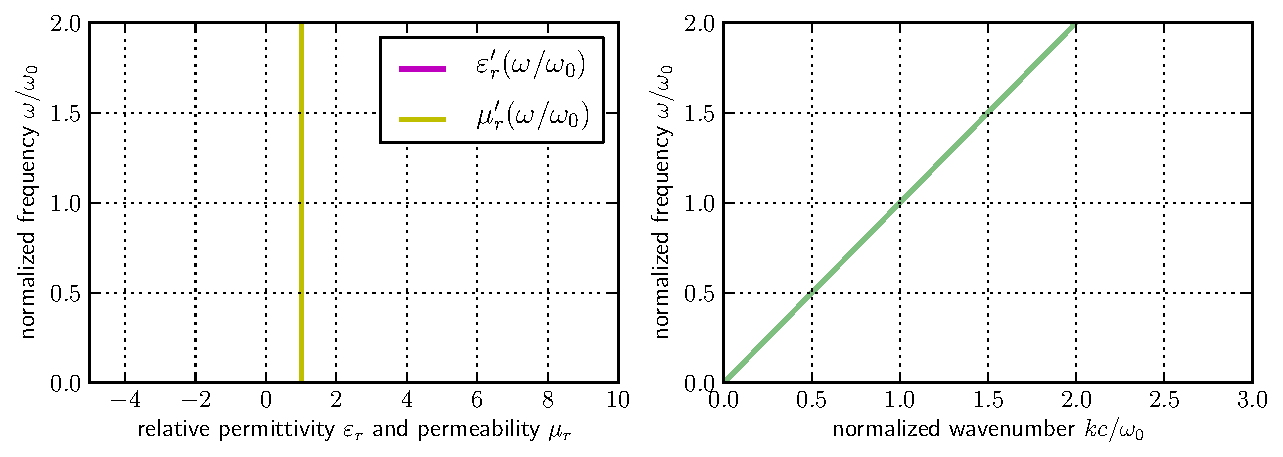
\includegraphics[width=\textwidth]{img/dispersion_landau_lifshitz/dispersion_vacuum.pdf}
\end{figure}
%}}}

\subsection{Local response of media to the electromagnetic field} \label{loc_response_of_media}
\paragraph{Local response definition} \label{subsection_local_resp} %{{{
In the whole chapter, we expect the medium properties to be time-invariant, linear, and homogeneous (i.e. independent of time, field amplitude and position in space, respectively). 
In this section, we focus on the special case when the response of the medium in point $\rr$ is not influenced by the electric field in any other point $\brho \neq \rr$. The medium is then said to be \textit{local}. 
For most media found in nature, this approximation is very close to reality and thus numerous electrodynamics textbooks tend to omit the nonlocal effects. 
However using this local theory to a wave propagating through periodic structures has a priori no justification and may lead to completely wrong results. The local theory presented here will serve as a basis for the nonlocal theory developed in following chapters.
% Applying the more familiar local electrodynamics to these structures is a mistake common to many papers. While the local theory is mathematically consistent, it predicts unusual spectral shapes and does not allow their further physical interpretation.

When an electric field $\E$ is applied, the medium responds by a change of the electric displacement $\D$ in a characteristic way. 
The immediate response of vacuum from the right side of the constitutive equations (\ref{eq_ce}) remains unchanged, but the response of the matter adds a new term called \textit{electric polarisation}. The polarisation is not instantaneous, so it is generally expressed as a convolution of the \textit{response function} $\chi_e$ with the values of electric field in the previous time $\tau$:
\begin{equation} \D(t,\rr) = \varepsilon_0 \E(t,\rr) + \varepsilon_0 \int_{-\infty}^{t}\chi_e(t-\tau)\, \E(\tau,\rr)\,\mbox{d}\tau. \label{eq_loc_chi_convol}\end{equation}
Let us assume that a harmonic plane wave propagates through the medium, so $\E(t, \rr) := \E_0 \, e^{\ii\omega t - \ii\kk\cdot\rr}$, as given by Eq. (\ref{eq_pw}). This can be inserted in the above equation:
\begin{equation} \D(t,\rr) = \varepsilon_0 \E_0 \, e^{\ii\omega t - \ii\kk\cdot\rr} + \varepsilon_0 \int_{-\infty}^{t} \chi_e(t-\tau) \, \E_0 \, e^{\ii\omega \tau - \ii\kk\cdot\rr} \,\mbox{d}\tau. \label{eq_chi_convol_harm}\end{equation}
Substituting $T:=t-\tau$, the exponent can be separated into two parts: one of which factors out of the integral, and one which turns the convolution into a temporal Fourier transform of the medium response:
$$				 \D(t,\rr) = \varepsilon_0 \E_0 \, e^{\ii\omega t - \ii\kk\cdot\rr} + \varepsilon_0 \int_{-\infty}^{0} \chi_e(T) \, \E_0 \, e^{\ii\omega (t - T) - \ii\kk\cdot\rr} \,\mbox{d}T,$$
$$				 \D(t,\rr) = \varepsilon_0 \E_0 \, e^{\ii\omega t - \ii\kk\cdot\rr} + \varepsilon_0 \left( \int_{-\infty}^{0} \chi_e(T)  \, e^{-\ii\omega T}\,\mbox{d}T  \right) \E_0 \, e^{\ii\omega t - \ii\kk\cdot\rr}.$$
This can be viewed as an application of the convolution theorem: convolution in time domain is equivalent to multiplication the in frequency domain.  %% FIXME normalisation by 2pi?
Consequently, we may introduce the local \textit{relative permittivity}, or also \textit{dielectric function}, $\epsrl(\omega)$ as a function of frequency. It is a property of the medium that determines how strongly it develops the electric displacement $\D$ in response to the electric field $\E$ of a harmonic wave.
From Eq. (\ref{eq_ce}) it is clear that in vacuum,  $\epsrl = 1$. In the medium, the permittivity may be obtained as
\begin{equation}  \epsrl(\omega) = \left.\frac{\D(t,\rr)}{\varepsilon_0 \E(t,\rr)} \right|_{\E(t, \rr) := 1 + \chi_e(\omega) = \E_0 \, e^{\ii\omega t - \ii\kk\cdot\rr}} = 1 + \int_{-\infty}^{0} e^{-\ii\omega T} \,\chi_e(T) \,\mbox{d}T. \label{eq_eps_loc}\end{equation}

In general, the function $\epsrl(\omega)$ is complex to account for possible phase delay between the harmonic driving field and the medium response. Phase delay different than $0$ (or integer multiple of $\pi$) corresponds to energy being dissipated in the medium.
Let us note that the definition of the Fourier transform is never subject to the sign change, even when the convention of $e^{\ii \omega t}$ is exchanged for $e^{-\ii \omega t}$.
%}}}
\paragraph{Response of a harmonic oscillator} \label{chap_lorentzmedia} %{{{
\begin{figure}[t] \caption{\textbf{a)} Illustration of how a simplified medium respond to an electric field impulse in the shape of Dirac delta function  $E(t) = \delta(t)$. The response is composed from an instantaneous part from vacuum, $\delta(t)$, and from a delayed ringdown of one damped harmonic oscillator, described by $\chi_e(t) := 2\pi \sin(2\pi t)\,e^{-x/2}$; \textbf{b)} The corresponding local permittivity $\epsrl(\omega)$, computed by Fourier transform of the response. Note that the imaginary part of permittivity is negative due to that the material is lossy (absorbs energy) and that the $e^{\ii\omega t}$ convention is used.} \label{fg_oscillator_spectrum} \centering 
	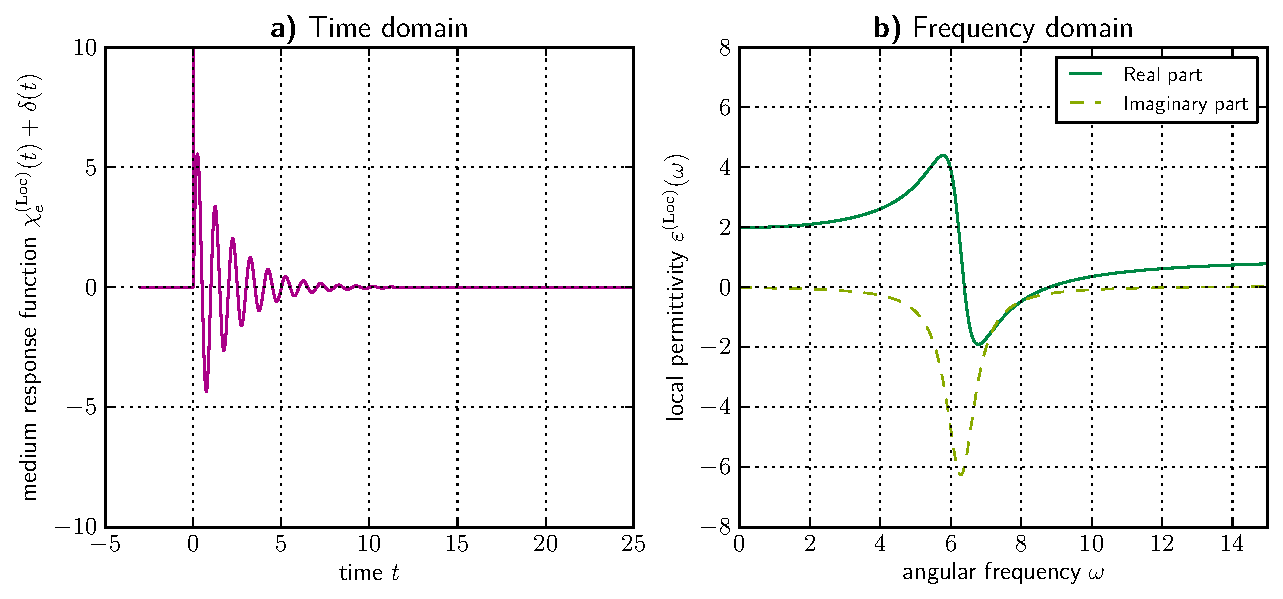
\includegraphics[width=\textwidth]{img/oscillator_spectrum.pdf}
\end{figure}
The response function $\chi_e(T, \mathbf{R})$ of usual media is composed of different phenomena.  Each of them may react on a different time scale, thus the response of the medium usually has a relatively complicated shape in the time domain.  However, to a reasonable degree of approximation, each of the contributions can be treated separately, as is demonstrated in the following.

Linear physical systems with an inertial mass, friction force and a restoring force are known as \textit{damped harmonic oscillators}.  This theory applies well to the electrons elastically bound to an atomic nucleus, as well as to the atoms elastically bound to their equilibrium positions in the lattice. The molecular rotations can also be modelled as (possibly overdamped) harmonic oscillators. Even free electrons in conductive media can fit into the theory of a harmonic oscillator provided the restoring force is set to nearly zero. The response of a harmonic oscillator is easy to describe both in time and frequency domains, even without the explicit use of the Fourier transform from Eq. (\ref{eq_eps_loc}). The harmonic oscillator model thus becomes a convenient starting point to approximate the response of materials.

A damped harmonic oscillator is described by a second-order differential equation:
\begin{equation} \alpha \frac{\partial^{2} x(t)}{\partial t^{2}} - \beta\frac{\partial x(t)}{\partial t} + \zeta x(t) = f(t). \label{eq_harm_osc}\end{equation}
Provided the driving term on the right hand side  is harmonic, $f(t) = e^{+\ii \omega t}$, the system response is also a harmonic function, $x(t) = \chi(\omega) e^{+\ii \omega t}$. The differential equation (\ref{eq_harm_osc}) can be easily solved to show that the complex amplitude of the driven oscillations, $\chi(\omega)$, depends on the angular frequency and on the positive real parameters $\alpha$, $\beta$ and $\zeta$ in the following way:
\begin{equation} \chi(\omega) \equiv \frac{x(t)}{f(t)} = \frac{1}{\zeta-\alpha\omega^{2} - \ii\omega\beta}  = \frac{\alpha^{-1}}{\frac{\zeta}{\alpha}-\omega^{2} - \ii\omega\frac{\beta}{\alpha}}. \label{eq_harm_osc_result}\end{equation}
The physical meaning of $\alpha$, $\beta$ and $\zeta$ is of little importance in this text, but without loss of generality the result of Eq. (\ref{eq_harm_osc_result}) can be rewritten into
\begin{equation} \chi(\omega) = \frac{F}{\omega_0^{2}-\omega^{2} - \ii\omega\gamma}, \label{eq_harm_osc_rewritten}\end{equation}
where the physical interpretation of the three (real and positive) parameters is as follows:
\begin{itemize}
 \item{$\omega_0 = \sqrt{\zeta/\alpha}$ is the angular \textit{resonance frequency}, at which the response is purely imaginary and usually its modulus $|\chi(\omega=\omega_0)|$ is near its maximum.} 
 \item{$\gamma = \beta/\alpha$ is the \textit{damping rate}. In time domain, it determines the time constant of exponential amplitude decay. In frequency domain, it is roughly proportional to the resonance width. } 
 \item{$F = \alpha^{-1}$ is the \textit{oscillator strength}, determining the amplitude of the response function.}
 \end{itemize}


\paragraph{Permittivity of Lorentz media} Within the approximation of relatively weak fields, the oscillators act independently of each other.
The response of usual media in frequency domain can thus be decomposed with acceptable precision into a sum of $Q$ independent harmonic oscillators, each $q$-th oscillator having the angular resonance frequency $\omega_{0q}$, damping rate $\gamma_q$ and strength $F_q$.
The permittivity function of the material is a solution of the differential equation of a damped harmonic oscillator, driven by a harmonic source:
\begin{equation} \epsrl(\omega) = 1 + \sum_{q=1}^Q \frac{F_q}{\omega_{0q}^2 - \omega^2 - \ii\omega\gamma_q} \label{eq_lorentz_eps}\end{equation} 
Advancing from the general formulation in Eq. (\ref{eq_eps_loc}) to the Lorentz oscillator model in Eq. (\ref{eq_lorentz_eps}) is of great importance for theoretical interpretation of the material response, and it has also become a framework for description of periodic structures even in the presence of spatial dispersion.  %% clumsy - remove this sentence?
A sample time- and frequency-domain response of a medium with one harmonic oscillator in is Fig. \ref{fg_oscillator_spectrum}.
% Note this is also the way how one communicates the material definition to the numerical simulation software, as described later (in Chap. \ref{chap_fdtd}). 

One can see that each oscillator increases the real part of the low-frequency permittivity, but in the high-frequency limit the contribution of the oscillator vanishes. This can be understood intuitively as that at low frequencies $\omega \ll \omega_0$, the system reacts fast enough to simultaneously follow the driving force, whereas at high frequencies  $\omega \gg \omega_0$, the system does not follow the driving force at all.
The contribution of one oscillator to the low-frequency permittivity $\Delta\epsrl(0)$, is inversely proportional to the oscillator restoring force, which links it to the inverse square of the resonance frequency:
\begin{equation} \Delta \epsrl'(\omega\rightarrow0) = \frac{F}{\omega_0^{2}}.  \label{eq_delta_eps} \end{equation}

A more detailed treatment of the theory of the permittivity $\epsrl(\omega)$ may be found in many textbooks, e.g. \cite[p. 454]{klingshirn2007semiconductor}, \cite{dresselhaus1966optical}. 

We will return to the Lorentz oscillator model also in the Chapter \ref{def_of_mat}, where it appears to be essential for realistic definition of materials for accurate numerical FDTD simulations. The chapter also describes in more detail how the overdamped molecular rotation and the unbound motion of free charges can be easily represented using correct parameters of an oscillator.
%}}}
\paragraph{Permeability}  %{{{ 
In a manner very similar to the above derivation of the local permittivity, the \textit{local permeability} can be introduced by means of a response of the medium to the magnetic field:
\begin{equation} \murl(\omega) = 1 + \chi_m(\omega) = \left.\frac{\B(t,\rr)}{\mu_0\HH(t,\rr)} \right|_{\HH(t, \rr) := \HH_0 \, e^{\ii\omega t - \ii\kk\cdot\rr}} = 1 + \int_{-\infty}^{0} e^{-\ii\omega T} \,\chi_m(T) \,\mbox{d}T, \label{eq_mu_loc}\end{equation}
where $\chi_m(T)$ is the \textit{magnetic response function} of the medium and $\HH_0$ is the amplitude of the magnetic field. This obviously results in an analogous expression for the local permeability in the frequency domain:
\begin{equation} \murl(\omega) = 1 + \sum_{q=1}^Q \frac{F_q}{\omega_{0q}^2 - \omega^2 - i\omega\gamma_q}, \label{eq_lorentz_mu}\end{equation} 
where formally the same notation was used as in  Eq. (\ref{eq_lorentz_eps}): $\omega_{0q}$, $\gamma_q$ and $F_q$ are here the magnetic oscillator's angular frequency, damping frequency and strength. Unlike the electric response, most ordinary media have either almost no response to the magnetic field or their response is limited to low frequencies.

%}}}
\paragraph{Kramers-Kronig relations in local media}%{{{
Causality prevents any medium from reacting to the future electric (or magnetic) field, so the integration in Eq. (\ref{eq_loc_chi_convol}) goes up to the current time only, $\tau \in (-\infty, t)$. The response of the medium to a real-valued field must moreover be also real, no matter that the computations are often done with complex field amplitude [Eq. (\ref{eq_pw})] for sake of convenience. 

Thus, the basic physical laws impose relatively strict constraints on the time-domain response function $f(t)$, which translate into other constraints for the possible shape of the response in frequency domain $F(\omega)$. The intuitive physical derivation is based on the fact that any time-domain response function can be trivially separated into its odd and even parts, as shown in Fig. \ref{fg_kk}. 
\begin{equation}f(t) = f_{odd}(t) + f_{even}(t) = -f_{odd}(-t) + f_{even}(-t) \label{eq_odd_even_decomp}\end{equation}
\begin{figure}[t] \caption{Illustration of how a real causal function $f(t)$ can be decomposed into the odd and even parts, which then yield a pure imaginary and pure real functions in the spectrum, respectively. Mathematically this is expressed in Eqs. (\ref{eq_odd_even_decomp}--\ref{eq_kkresult}).} \label{fg_kk} \centering 
	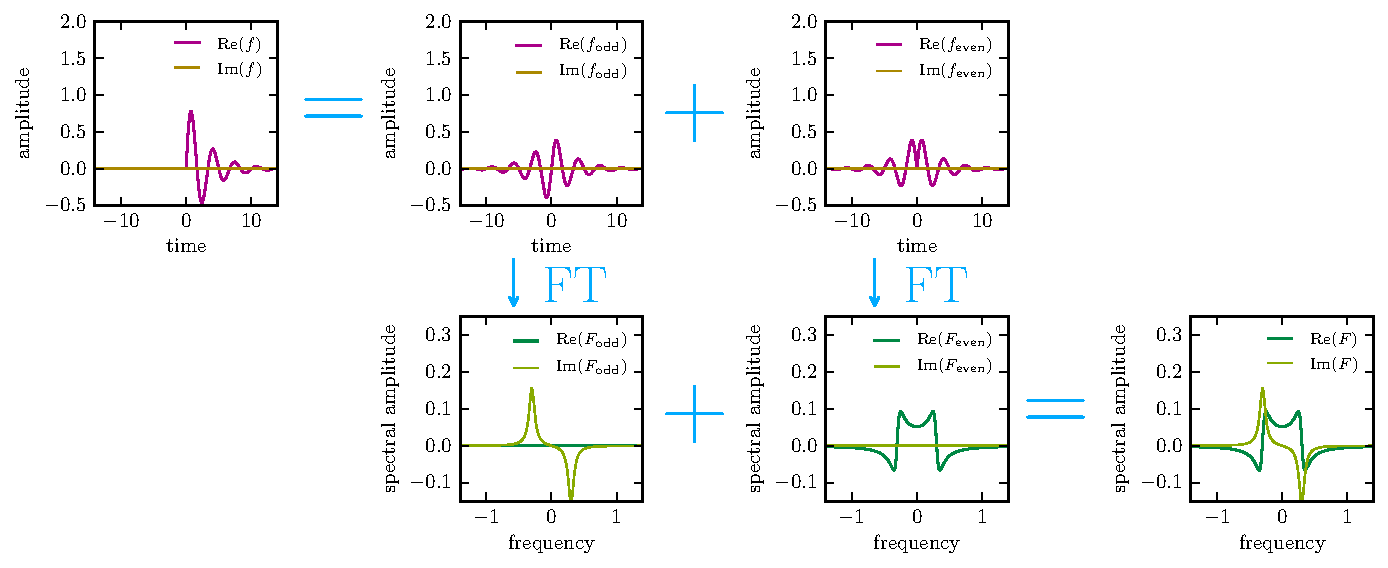
\includegraphics[width=17.5cm]{img/Kramers_Kronig_plot/kk.pdf}
\end{figure}
The Fourier transform of a real odd function is an imaginary function:
%F_{odd}(\omega)=& \int_{-\infty}^{\infty} e^{-\ii \omega t} f(t) \mbox{d}t = \\
		 %=&  \frac{1}{2} \int_{0}^{\infty} e^{-\ii \omega   t } [ f_{odd}(t) + f_{even}(t)] \mbox{d}t 
		   %+ \frac{1}{2} \int_{0}^{\infty} e^{-\ii \omega (-t)} [-f_{odd}(t) + f_{even}(t)] \mbox{d}t  \\
		 %=&  \int_{0}^{\infty} \frac{e^{-\ii \omega t}-e^{+\ii \omega t}}{2} f_{odd}(t) \mbox{d}t 
		   %+ \int_{0}^{\infty} \frac{e^{-\ii \omega t}-e^{+\ii \omega t}}{2} f_{odd}(t) \mbox{d}t  = \\
		 %=&\int_{-\infty}^{\infty} e^{-\ii \omega t} f(t) \mbox{d}t  = \\
		 %=&\int_{-\infty}^{\infty} e^{-\ii \omega t} f(t) \mbox{d}t  = \\
\begin{equation} 
\begin{split} 
F_{odd}(\omega)=& \int_{-\infty}^{+\infty} e^{-\ii \omega t} f_{odd}(t) \,\mbox{d}t = 
		 \int_{-\infty}^{+\infty} \frac{e^{-\ii \omega   t }}{2} f_{odd}(t) \,\mbox{d}t 
		   +  \int_{-\infty}^{+\infty} \frac{e^{-\ii \omega (-t)}}{2} [-f_{odd}(-t)] \,\mbox{d}t  \\
		 =&   \int_{-\infty}^{+\infty} \frac{e^{-\ii \omega t}-e^{+\ii \omega t}}{2} f_{odd}(t) \,\mbox{d}t 
		 = -\ii \underbrace{\int_{-\infty}^{+\infty} \sin(\omega t) \, f_{odd}(t) \,\mbox{d}t}_{\mbox{$\in \mathbb{R}$}},
\end{split} 
\label{eq_kkF}\end{equation}
whereas the Fourier transform of a real even function yields a real function:
\begin{equation} 
\begin{split} 
F_{even}(\omega)= \ldots =   \int_{-\infty}^{+\infty} \frac{e^{-\ii \omega t}+e^{+\ii \omega t}}{2} f_{even}(t) \,\mbox{d}t 
		 = \underbrace{\int_{-\infty}^{+\infty} \cos(\omega t) \, f_{even}(t) \,\mbox{d}t}_{\mbox{$\in \mathbb{R}$}}.
\end{split} 
%% is the following is WRONG?? see http://www.thefouriertransform.com/pairs/step.php#signum,  ho3.pdf
\label{eq_kkFeven}\end{equation}
The odd and even components of the time-domain response function correspond to the imaginary and real part of the response spectrum, respectively:
\begin{equation} F_{odd}(\omega) + F_{even}(\omega) = F(\omega), \text{ where } F_{odd}(\omega) = F''(\omega) \text{ and } F_{even}(\omega) = F'(\omega).  \label{eq_kkFodd}\end{equation}
At the same time, $f_{even}(t)$ and $f_{odd}(t)$ are related to each other by having the opposite sign for $t<0$ and the same sign for $t>0$, that is 
\begin{equation} f_{even}(t) = \mbox{sign}(t)\,f_{odd}(t). \label{eq_kkfeven}\end{equation}
The multiplication in the time domain translates into a convolution in the frequency domain
\begin{equation} 
F_{even}(\omega) = \int_{-\infty}^{+\infty}  \frac{-2\ii}{\omega - \Omega} F_{odd}(\omega) \,\mbox{d}\Omega  \equiv  \left[\frac{-2\ii}{\omega}\right]\,\ast\,F_{odd}(\omega),
\label{eq_kkresult}\end{equation} 
where we used the knowledge that the $-2\ii/\omega$ function is the Fourier transform of $\mbox{sign}(t)$. Convolution with this function is also known as the Hilbert transform. % tODO cite

Obviously, Eq. (\ref{eq_kkfeven}) can also be converted to $f_{odd}(t) = \mbox{sign}(t)\,f_{even}(t)$, thus the relation between the real and imaginary parts of the response spectrum also holds when $F_{odd}(\omega)$ and $F_{even}(\omega)$ are exchanged in Eq. (\ref{eq_kkresult}). 

A related mathematical proof of the Kramers-Kronig relations can be derived from the analyticity of the response function in the complex plane of frequency. \cite[p. 125]{klingshirn2007semiconductor}

% maybe:: why do K-K relations forbid to choose arbitrary phase difference over an unit cell? 
%     ... ie. Why the N_eff can be unambiguously extracted from spectra?
% maybe: show how it dictates the "constant area of imaginary part " when resonance Q is changed
%}}}

\subsection{Dispersion relations in local Lorentz media} \label{disp_rel_local_media}
\paragraph{Lower and upper polariton branches of transverse waves} %{{{
Returning to the derivation of dispersion relations, we start with modifying the constitutive relations (\ref{eq_ce}) to a plane wave propagating in a medium:
\begin{equation}		\D := \varepsilon_0\epsrl(\omega)	\E, \quad\quad\quad						\B := \mu_0\mu_r(\omega)		\HH,				 \label{eq_ce2}\end{equation}
with the relative permittivity $\epsrl(\omega)$ and permeability $\mu_r(\omega)$ being two dimensionless functions of frequency, defined in Eq. (\ref{eq_lorentz_eps}, \ref{eq_lorentz_mu}). 
The wave equation (\ref{eq_wavek}) then changes to
\begin{equation}  \TT\E = \varepsilon_0 \mu_0  \epsrl(\omega) \murl(\omega) \, \frac{ \omega^{2}}{k^2} \E.  \label{eq_wavek_disp}\end{equation}
For transverse waves in isotropic media, the electric field is perpendicular to the wave vector ($\TT\E = \E$), and Eq. \ref{eq_wavek_disp} can be simplified to  
\begin{equation} k(\omega) = \sqrt{\varepsilon_0 \mu_0} \sqrt{\epsrl(\omega) \mu_{r}(\omega)}\;\omega = \sqrt{\epsrl(\omega) \mu_{r}(\omega)}\; \frac{\omega}{c}, \label{eq_dispeq_loc}\end{equation}
with the added frequency-dispersive term responsible for the deviation of the curve in Fig. \ref{fg_dcsimpleel} from the original straight light line in Fig. \ref{fg_dcvac}. 

In the simplest example of a single electric resonance with negligible losses, as shown in Fig. \ref{fg_dcsimpleel}, the curve is divided into two separate branches. The \textit{lower polariton branch} is below the resonance frequency $\omega_0$ and it is characterized by the Lorentz oscillator being in phase with the electric field. Above $\omega_0$, the dipoles of the Lorentz oscillator can no more follow the electric field and point in the opposite direction. With further increase of the frequency, the permittivity crosses zero at the frequency $\omega_{\text{L}}$ where the \textit{upper polariton branch} starts. In case of a single (or well-isolated) Lorentz oscillator, the difference $\omega_{\text{L}} - \omega_0$ can be computed from the magnitude of the oscillator (using the Lydanne-Sachs-Teller relation) \cite{klingshirn2007semiconductor}.

The same behaviour is observed for a single resonance in the permeability $\mu_r(\omega)$, and will be typical also of the spectra of resonances of macroscopic structures described later.

Note that the formation of upper and lower polariton branches can be reinterpreted\cite{landau1984electrodynamics} using the theory of coupled oscillators as the result of \textit{anticrossing} between the oscillator at the frequency $\omega_0$ (forming a horizontal line) and the photon branch (forming a straight growing light-line). \label{anticrossing}

When losses are present, the lower and upper polariton branches (in Fig. \ref{fg_dcsimpleel}) are connected by a smooth line of \textit{anomalous} dispersion and very high losses.  

%}}}
\paragraph{Longitudinal waves in dispersive media} %{{{
The wave equation in local dispersive media (\ref{eq_wavek_disp}) 
%\begin{equation} - \kk (\kk \cdot \E) + k^2 \E = \varepsilon_0 \epsrl(\omega) \mu_0 \murl(\omega) \omega^{2} \E, \tag{\ref{eq_wavek_disp} \again} \end{equation}
also allows the existence of longitudinal waves with electric field parallel to the wave vector $\E || \kk$. It was shown earlier that there is no solution for longitudinal waves in vacuum except for a static homogeneous field.

\begin{figure}[t] \caption{Influence of a single resonance in the real part of relative permittivity $\epsrl'(\omega)$ (magenta curve in the left panel) to the shape of dispersion curves in the right panel (green curve, computed using Eq. (\ref{eq_dispeq_loc}). The lower and upper polariton branches are separated by a spectral region $\omega \in (0.3, 0.65)$, where the wave does not propagate on an appreciable distance (nonzero losses yield a finite solution here, though).} \label{fg_dcsimpleel} \centering 
	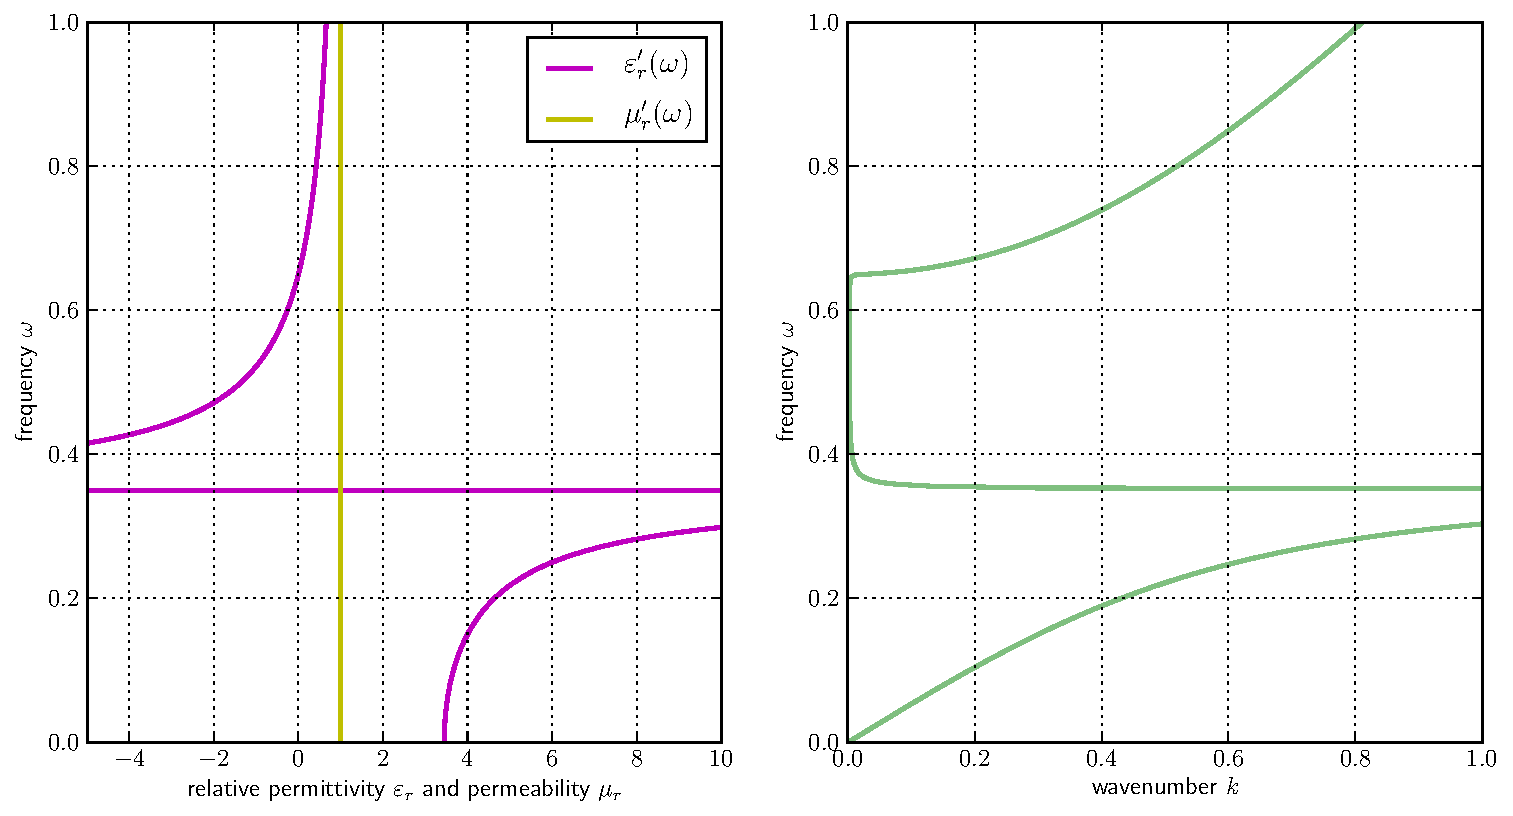
\includegraphics[width=\textwidth]{img/dispersion_landau_lifshitz/dispersion_simple_el.pdf}
\end{figure}
If a local medium is assumed, and the wavenumber $k$ is nonzero, such waves can have a solution with nonzero $\E$ when $\epsrl(\omega)' = 0$, or with nonzero $\HH$ when $\mu_r(\omega)' = 0$. Therefore, the corresponding dispersion curve for a longitudinal wave is a horizontal line at $\omega = \omega_{\text{L}}$, independent of $k$. This would be equivalent to a standing oscillation that maintains the spatial amplitude envelope that was originally excited. 

Different physical phenomena can lead to $\epsrl(\omega)' = 0$, some of which introduce relatively low losses at the corresponding $\omega_{\text{L}}$; namely lattice vibrations in nonconductive crystals or electrons in inductive media (like metals and dilute plasma). 

At the interface of two media with differing signs of permittivity, another type of waves can be excited with an intermediate frequency $\omega < \omega_{\text{L}}$ that can not propagate in either of the bulk medium. The dispersion curve of such waves is not flat, allowing them to propagate along the interface. Depending on the mechanism, they are known as  \textit{surface plasmons} or \textit{surface phonon-polaritons} \cite[p. 87]{klingshirn2007semiconductor}, respectively. Accordingly, \textit{surface magnons} should be observed at interfaces where $\mu$ changes its sign.
% Are there surface magnons?
% Are there any metamaterials designed for longitudinal waves?
%}}}
\paragraph{Anisotropy of permittivity} \label{par_anisotropy} %{{{
It shall be noted here that the permittivity $\epsrl$ was introduced as a scalar, assuming that the vector of electric field $\E$ and electric induction $\D$ are always parallel:
\begin{equation} \D = \varepsilon_0 \epsrl(\omega) \E \equiv \varepsilon_0  
	\left(\begin{array}{ccc} 
			\epsrl(\omega) & 0 & 0  \\
			0 & \epsrl(\omega) & 0  \\
			0 & 0 &\epsrl(\omega)  
	\end{array} \right) \cdot \E
	\label{eq_ed_orientation}
\end{equation}
In some media with a lower rotational symmetry (such as many crystals, or liquids under static electric field), the medium response depends on the electric or magnetic field direction, and the medium is denoted as \textit{anisotropic}. At the beginning of the chapter we assumed the fields to be relatively weak, which enables one to describe the medium as \textit{linear}. Whatever the linear relation of $\D := \mathcal{L}(\E)$, it must obey the rule
$$\D_1 + \D_2 = \mathcal{L}(\E_1) + \mathcal{L}(\E_2) = \mathcal{L}(\E_1 + \E_2)$$
for any vectors $\E_1, \E_2$. Such a relation can be fully described by a \textit{tensor of permittivity} 
\begin{equation} \D = \varepsilon_0 \epsrl(\omega) \E \equiv \varepsilon_0  
	\left(\begin{array}{ccc} 
	{\epsrl}_{xx}(\omega) & {\epsrl}_{xy}(\omega) & {\epsrl}_{xz}(\omega)  \\
	{\epsrl}_{yx}(\omega) & {\epsrl}_{yy}(\omega) & {\epsrl}_{yz}(\omega)  \\
	{\epsrl}_{zx}(\omega) & {\epsrl}_{zy}(\omega) & {\epsrl}_{zz}(\omega)  
	\end{array} \right) \cdot \E.
	\label{eq_epstensor}
\end{equation}
An elaborate discussion on all possible forms of this tensor and their physical interpretations can be found e.g. in \cite[pp. 678--686]{born1999book}. An analogous treatment can be applied to the magnetic permeability, though it is less often needed.

%}}}
\paragraph{Dispersion relations in anisotropic local media}  %{{{
If the medium response depends on the direction of the field, the dispersion relations can not be directly obtained by substitution into the wave equation as in Eq. \ref{eq_dispeq_loc}.
% a linear transformation of the vector $\E$, which can be expressed by the tensor
%$$ - \kk (\kk \cdot \E) \equiv 
	%-\left(\begin{array}{c} k_x \\ k_y \\ k_z \end{array} \right) \cdot
	%\left[\left(\begin{array}{ccc} k_x & k_y & k_z \end{array} \right) \cdot
	%\left(\begin{array}{c} E_x \\ E_y \\ E_z \end{array} \right)\right] 
		%\equiv
	%\left(\begin{array}{ccc} -k_x^2 & -k_x k_y & -k_x k_z \\ -k_y k_x & -k_y^2 & -k_y k_z \\ -k_z k_x & -k_z k_y & -k_z^2 \end{array} \right) \cdot  
	%\left(\begin{array}{c} E_x \\ E_y \\ E_z \end{array} \right).
	%$$
%$$ k^2 \E \equiv 
%	\left[\left(\begin{array}{ccc} k_x & k_y & k_z \end{array} \right) \cdot 
%	\left(\begin{array}{c} k_x \\ k_y \\ k_z \end{array} \right)\right] \cdot 
%	\left(\begin{array}{c} E_x \\ E_y \\ E_z \end{array} \right),
%	$$
%$$ \mu_0 \varepsilon_0 \omega^{2} \E \equiv 
%	\left(\begin{array}{ccc} k_x^2+k_y^2+k_z^2 & 0 & 0 \\ 0 & k_x^2+k_y^2+k_z^2 & 0 \\ 0 & 0 & k_x^2+k_y^2+k_z^2 \end{array} \right) \cdot  
%	\left(\begin{array}{c} E_x \\ E_y \\ E_z \end{array} \right),
%	$$
The dispersion relation can however still be solved \cite[pp. 667]{born1999book} as a set of three linear algebraic equations based on Eq. (\ref{eq_wavek_disp}).
%\begin{equation} \left|\begin{array}{ccc} 
	%k_y^2+k_z^2 - \mu_0 \varepsilon_0 \omega^{2} 		& -k_x k_y 		& -k_x k_z \\ 
	%-k_y k_x 		& k_x^2+k_z^2-\mu_0\varepsilon_0\omega^{2} 		& -k_y k_z \\ 
	%-k_z k_x 		& -k_z k_y		& k_x^2+k_y^2-\mu_0\varepsilon_0\omega^{2}
	%\end{array} \right| = 0, \label{eq_dispdet}\end{equation}
For simplicity, we assume here that the relative permeability $\murl = 1$; the extension to other cases is possible, too. %% TODO Do epsilon and mu commute, if they are both tensors??
A solution of Eq. \ref{eq_wavek} can exist with nonzero $\E$ if and only if the determinant of the set of three linear equations is zero:
\begin{equation} 
\det\left[
\TT -
	\frac{\mu_0 \varepsilon_0 \omega^2}{k^2}
	\left(\begin{array}{ccc} 
	{\epsrl}_{11}(\omega) & {\epsrl}_{21}(\omega) & {\epsrl}_{31}(\omega)  \\
	{\epsrl}_{12}(\omega) & {\epsrl}_{22}(\omega) & {\epsrl}_{32}(\omega)  \\
	{\epsrl}_{13}(\omega) & {\epsrl}_{23}(\omega) & {\epsrl}_{33}(\omega)  
	\end{array} \right) \right] = 0, \label{eq_dispdet}\end{equation}
The search for dispersion curves in an anisotropic medium is thus transformed into finding zeroes of this function of four scalar variables, $k_x$, $k_y$, $k_z$ and $\omega$.
In the most general case, it can be solved by means of numerical algebra software. 
%It would be nice to write about the number of solutions

%}}}
\paragraph{Isofrequency contours}  %{{{
%A resonance in local permittivity (or permeability) creates two polariton branches -- thus the dispersion curves can not be expressed as one simple function $\omega(k)$ of the wavevector $k$. It would then appear adequate to treat dispersion curves as a function of frequency, $k(\omega)$, but as is shown below in the presence of nonlocal response, neither $k$ is necessarily a simple function of $\omega$. Also 
It is often important to describe the dispersion curves also for different wave angles, which is the best accomplished by plotting the % (real part of)
frequency $\omega$ as the function of \textit{wave vector} $\kk$. In three dimensions, this would require mapping a function of three independent variables, $\omega(\kk) = \omega(k_x, k_y, k_z)$. However, in most cases the projection of two selected components of $\kk$ is sufficient to understand all relevant phenomena, and naturally it is much easier to visualize. 
\begin{figure}
  \begin{minipage}[c]{0.5\textwidth}
\hfill
    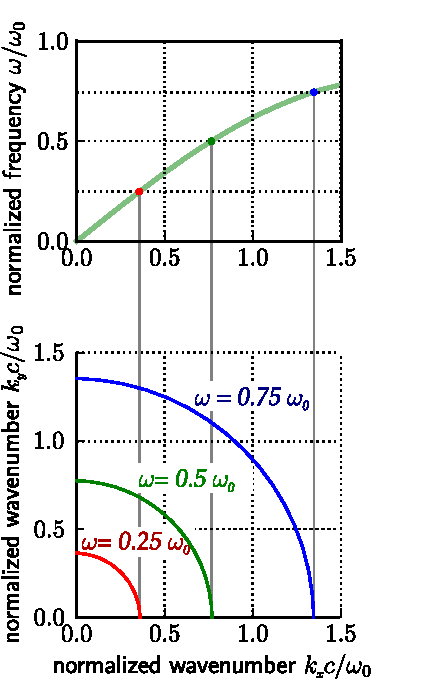
\includegraphics[width=7cm]{img/dispersion_curves_to_ifc.pdf}
  \end{minipage}
  \begin{minipage}[c]{0.5\textwidth}
    \caption{Relation between a dispersion curve for one photonic branch and the corresponding isofrequency contours. At a selected frequency, all points in the $k_x$-$k_y$ plane are drawn for which a nonzero solution of Maxwell equations exists. For transverse waves in local media, this is equivalent to finding a solution to the dispersion equation (\ref{eq_dispeq_loc}).\\Multiple frequencies can be plotted to describe the frequency dependence. For illustration, an isotropic medium was used, thus all IFCs take the form of a circle. To save space, only one quarter of the circle was plotted here.} \label{fg_ifc_dc}
  \end{minipage}
\end{figure}

Such plots are known as \textit{isofrequency contours} (IFC), or also \textit{equifrequency contours} (EFC), and they allow intuitive geometrical analysis of various phenomena such as light refraction, beam walk-off, total internal reflection etc. 
The relation between a dispersion curve for one photonic branch and the corresponding isofrequency contours in an isotropic medium is illustrated in Fig. \ref{fg_ifc_dc}.

The limitation is, however, that IFC plots do not show the imaginary part and thus are applicable to plot the dispersion in media with no or negligible losses only.  
Each photonic branch also has to be plotted in a separate plot to prevent the contours from overlapping (see the right panel of Fig. \ref{fg_dcsimpleel}). 
Moreover, in every single photonic band, Eq. \ref{eq_dispdet} yields two solutions for two possible polarisations of transverse waves \cite[p. 46]{klingshirn2007semiconductor}. The IFCs for these solutions are in general different in anisotropic media, but we always restrict the discussion only to one polarisation in the following figures for simplicity. 
% discuss this further? In uniaxial media, where two diagonal components ...

\begin{figure}[ht] \caption{\textbf{(a)} Isofrequency contours for an isotropic medium are circular and centered in the $k=0$ point. \textbf{(b)} An anisotropic medium with the optical axis perpendicular to the interface, where IFCs take the form of ellipses. \textbf{(c)} A similar case of another anisotropic medium, with the orientation of the optical axis (drawn as the dashed black line) that enables to introduce the index of refraction for the shown direction of the wave vector $\kk$. In the plots (b) and (c), the IFCs are plotted for one polarisation only.
%% FIXME \textbf{(d)} A dispersive \textit{hyperbolic medium}, with one component being a function of frequency and crossing zero.
} \label{fg_ifc} \centering  %% TODO verify in Belov that local media may be used as hyperbolic
	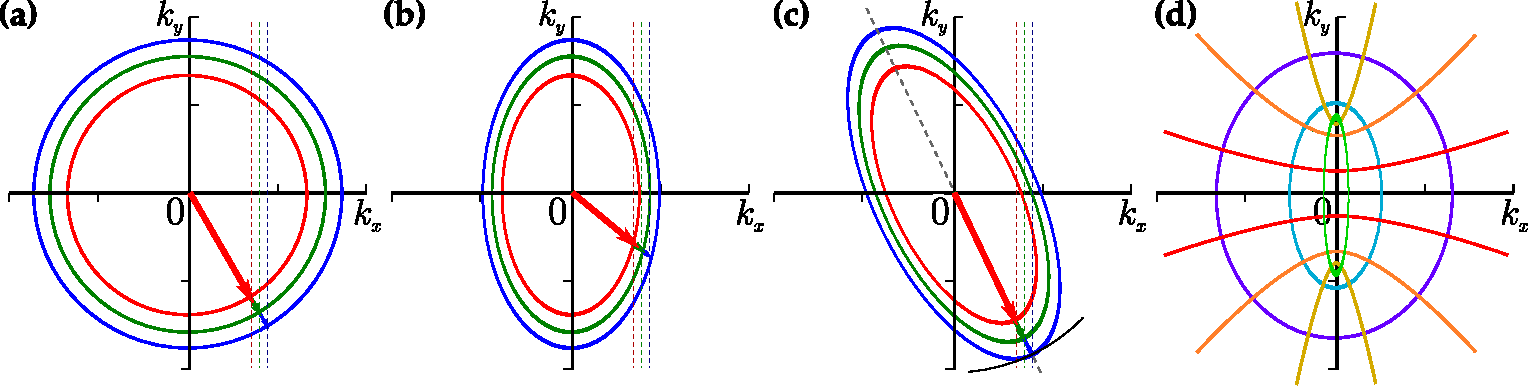
\includegraphics[width=.8\textwidth]{img/ifc_freqdispersion.pdf} 
\end{figure}
IFCs are valuable for graphical prediction of wave refraction on interface of two media \cite[p. 118]{shalaev2010book}. Starting, e.g., by an isotropic medium in Fig. \ref{fg_ifc}a, the wavevectors are known for given frequencies (as three coloured arrows).
The component of wave vector parallel to the interface (chosen as $k_x$ here and indicated by the vertical dashed lines) must be conserved upon refraction. This rule can be intuitively deduced from the continuity of the wave phase at the interface, as well as from the Noether theorem applied to the infinite translational symmetry of the interface. Transferring the vertical dashed lines to an IFC plot of another medium and finding the intersections with an IFC of the corresponding frequency, one can find the new wavevector. 
In Fig. \ref{fg_ifc}, we provide examples of IFCs for one isotropic and two anisotropic media.

%}}}
\paragraph{Index of refraction and its applicability}  %{{{
With the background of the theory developed above, the notion of the \textit{index of refraction} $N$ can be properly introduced and discussed. 
In the strictest sense, the index of refraction is defined only for \textit{isotropic} media. Then it is equivalent to the ratio of the wavenumber $k(\omega) \equiv |\kk|$ to the wavenumber in vacuum at the same frequency: 
\begin{equation} N(\omega) := k(\omega) \, \frac{c}{\omega} \equiv \sqrt{\epsrl(\omega)\murl(\omega)}, \label{eq_dispeqN}\end{equation}
as directly follows from Eq. (\ref{eq_dispeq_loc}).

Starting with a harmonic plane wave with the frequency $\omega$ and the wave vector $\kk^{(1)}$ refracting at an interface of two isotropic media, the projection of $\kk^{(1)}$ to the interface is given as 
$$ k_x = k^{(1)}\,\sin \alpha^{(1)}, $$
where $\alpha^{(1)}$ is the angle between the wavevector in the first medium $\kk^{(1)}$ and the  normal to the interface. In the second medium, a similar relation must apply. Therefore, the wavenumber $k^{(2)}$ may be different and as a result, the angle in the second medium is
\begin{equation} \alpha^{(2)} = \arcsin\left( \frac{k^{(1)}}{k^{(2)}} \,\sin \alpha^{(1)} \right) = \arcsin\left( \frac{N_1}{N_2} \,\sin \alpha^{(1)} \right), \label{eq_snell}\end{equation}
which is known as the \textit{Snell} (or also \textit{Snell-Descartes}) law.

The majority of (effective) media discussed in this thesis are, however, more or less anisotropic, and somewhat surprisingly, the notion of \textit{index of refraction} $N$ seems to be widely used for them in the literature anyway. The author thus feels there is a need for a conscientious extension of $N$ for anisotropic cases, too. An extremely loose definition of $N$ could be based on computing the ratio $N(\omega, \kk) := kc/\omega$  for any medium. This can be formally done, but then the wavenumber $k$ would also depend on the direction $\alpha$, and the Snell law in Eq. (\ref{eq_snell}) would become an implicit equation, losing its original purpose of making the computation explicit and notably simple.

The author proposes instead to restrict the term \textit{index of refraction} to all cases where IFCs are perpendicular to $\kk$. This covers not only all isotropic media, but also those cases when the waves propagate close the optical axis of any anisotropic media. An example of an anisotropic medium with its optical axis oriented in such a way that the refraction can be computed using Snell law provided the $k_x$ component is shared with \ref{fg_ifc}a, is shown in Fig. \ref{fg_ifc}c. For small deviations from this angle, where the IFC can be approximated by an osculating circle, 
\begin{equation} \frac{\partial k}{\partial \alpha} \ll k,\label{eq_osculating}\end{equation}
the Snell law still gives a correct prediction of the refraction angle. 

We will show in the following that the prediction of \textit{beam} propagation is more complex, because it is sensitive to the \textit{curvature of IFCs}. 

%}}}
%%   \paragraph{Isofrequency contours of hyperbolic media}  %{{{ todo? add from Belov2003 
%%   The IFCs in Fig. \ref{fg_ifc}a,b,c were plotted for non-dispersive media, i. e. with $\epsrl$ and $\murl$ independent of frequency. The case of one polariton branch of a dispersive isotropic medium is already shown in Fig. \ref{fg_ifc_dc}, characteristic by non-equidistant IFCs which lead to the refraction angle being dependent on the frequency.
%%   
%%   A more complicated cases are the \textit{hyperbolic media}, where, in a certain spectral region, one component of the anisotropic permittivity is positive, while another one is negative. The solution of Eq. (\ref{eq_dispdet}) then results in a hyperboloid, which is either of one sheet or two sheets, depending on the sign of the remaining diagonal component of permittivity tensor. At the frequencies where the dispersive component of permittivity is negative,  
%%   Note that a negative permittivity is always connected with the dispersive behaviour, thus \ref{fg_ifc}d is another example of a dispersive medium. 
%%   
%%   %}}}
\paragraph{Group velocity}  %{{{  
So far, only the propagation and refraction of a plane harmonic wave was discussed, and it was shown that it is determined by the shape of IFC at the given frequency.
Temporal modulation of the wave 
% can be expressed by a complex vector function $\E_0(t)$ that replaces the constant vector $\E_0$ in Eq. \ref{eq_pw}. This 
is equivalent to the wave being formed by superposition of multiple frequency components in the frequency domain, with their respective amplitudes given by the Fourier transform of the field envelope. The temporal position of the envelope in is determined by their \textit{mutual phase difference}, not by the absolute wave phase. 
%redund As a special case, when all components propagate with the same velocity, the envelope does not shift against the wave phase. 

A similar argument can be made with regards to the spatial modulation of the wave. Any wave shape other than the infinite plane wave is a superposition of waves with different wavevectors, and the direction of propagation of its spatial envelope is given by mutual phase difference of the constituent waves. % TODO rewrite-unclear

The velocity vector of the envelope propagation, denoted as the \textit{group velocity} $\vg$, can be found as the gradient of frequency by the wavevector: %% TODO cite
\begin{equation} \vg := \frac{\partial \omega}{\partial \kk} \equiv 
\left(\begin{array}{c} 
	\partial \omega/\partial k_x \\ 
	\partial \omega/\partial k_y \\ 
	\partial \omega/\partial k_z \\ 
	\end{array} \right)
 \label{eq_vg}\end{equation}
In the IFC plot, the group velocity can be found visually as directing always perpendicular to the IFC, with a magnitude being proportional to the density of the IFCs.

If the group velocity is different from the phase velocity, the envelope $\E_0(t)$ is maintained in time, but it continuously shifts against the underlying wave. Thus the actual temporal shape of $\E(t)$ changes upon passing through a dispersive medium.
On the contrary, in vacuum or media with negligible dispersion, each frequency component of the wave acquires an additional phase strictly proportional to its frequency. Then the group velocity coincides with the phase velocity: 
$$\hspace{3cm}\vg = \kk \omega / k^2 \hspace{3cm} \text{(in nondispersive isotropic media)}.$$
%The orientation of $\vg$ and $\kk$ is usually the same, but later it will be shown that it can be otherwise, with peculiar physical consequences.

Usually, in spectral regions near a resonance, also the quadratic or even higher terms in the Taylor expansion of the $\omega(\kk)$ dependence shall be taken into account. This effect is known as the \textit{group velocity dispersion} as it is equivalent to the group velocity $\vg(\kk)$ being dependent on the wavevector (or, if reformulated, on frequency). It results in a temporal distortion of the wave envelope $\E_0(t)$.  %% TODO ... and what about the wave distortion in space?
%}}}
\paragraph{Beam propagation in anisotropic media}  %{{{  
The refraction of a beam is illustrated in Fig. \ref{fg_ifc2} by means of three slightly different wavevectors it is composed of. For simplicity, a monochromatic wave was used, so brown, black and violet were chosen for the three example wavevectors to prevent confusion with the rainbow-like frequency color map used in Fig. \ref{fg_ifc}. 

In the first plot, \ref{fg_ifc2}a, the case of an isotropic medium is illustrated. Upon refraction into a general anisotropic medium in Fig. \ref{fg_ifc2}b, each component must maintain its wavevector projection to the interface, thus the wavevectors spread in their direction. The resulting beam propagates along the group velocity that is different from the central wavevector; % The components of the resulting beam are   is narrower and does not propagate 
this is also known as the spatial \textit{walk-off}.
\begin{figure}[ht] \caption{Examples of IFCs similar to Fig. \ref{fg_ifc}, but now at a single frequency and different wavevectors, corresponding to a monochromatic beam refracting on the interface. \textbf{(a)} The wavevectors in the isotropic medium lie on a circle.
		\textbf{(b)} Generally, anisotropic media exhibit different orientations of the wave vector $\kk$ and the beam propagation. \textbf{(c)} For the special cases of propagation along the optical axis, the beam refracts similarly as in isotropic media.
 \textbf{(d)} In anisotropic media with hyperbolic shape of the IFC, the beam refracts to the opposite direction than the wave vector. } \label{fg_ifc2} \centering 
	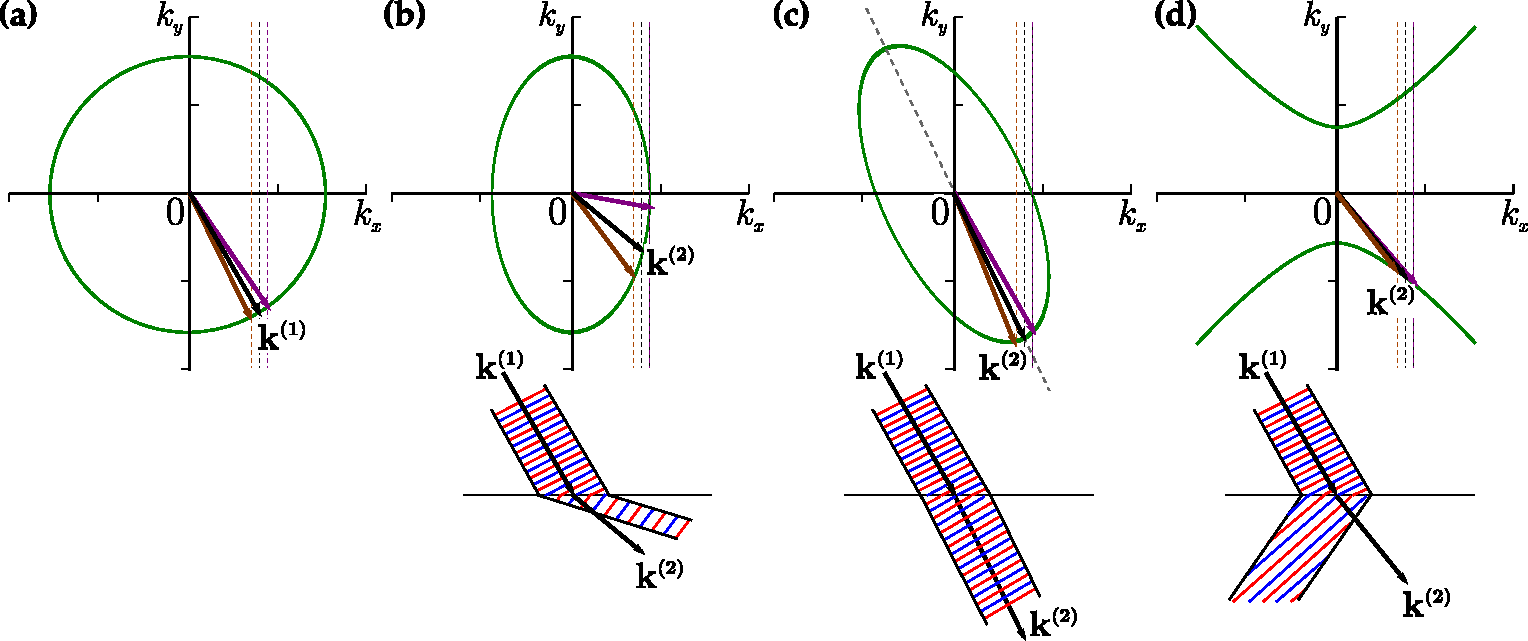
\includegraphics[width=\textwidth]{img/ifc_kdispersion_hyp.pdf} 
\end{figure}

Fig. \ref{fg_ifc2}c shows again the special case of the anisotropic medium, where the wave propagates near an optical axis, and thus where the Snell law can still be used to determine the refraction of a plane wave, based the generalized notion of the index of refraction.
However, there is a pitfall if one tries to apply the Snell law for prediction of how the beam will refract. The problem originates from the differential nature of the group velocity definition in Eq. (\ref{eq_vg}). 
%While the magnitude of the wavevector changes only negligibly, with the square of a 
While the phase velocity of a monochromatic wave at the frequency $\omega_0$ does not appreciably change upon a small deviation of the angle $\alpha$ from the optical axis  [c.f.  Eq. (\ref{eq_osculating})], the group velocity direction does, because it has a nonzero linear component in its dependence on the wavevector:
$$ \frac{\partial \vg(\kk)}{\partial \alpha} \neq 0.$$
As a result, the group velocity in anisotropic media is always much more sensitive to the angle than the phase velocity, and Snell law does not predict it correctly. It can be regarded as a spatially-dependent manifestation of the group velocity dispersion.

In Fig. \ref{fg_ifc2}d, an extreme case of spatial walk-off is shown on the example of a \textit{hyperbolic} medium with different signs of the permittivity along different axes. %% TODO study Belov2003 and possibly correct this if hyperbolas are wrong
 The normal to its IFC is nearly perpendicular to the wavevector, and accordingly, the beam refracts in opposite angle with regards to the incident wave. The $k_x$ component of the wave vector is however still maintained. A further geometrical development of the beam refraction is in Ref. \cite[p. 46]{klingshirn2007semiconductor}.

%If the amplitude and phase of the wave is not  temporal shape of a wave can be composed as a superposition of different frequency components with certain amplitude and phase. Similarly, any spatial shape of a beam can be composed of infinite waves of different wavevectors. The isofrequency contours, and their dependence on frequency, allow to determine how the temporal and spatial envelope will propagate. 
%Assuming a short pulse for simplicity

%}}}
\paragraph{The sign of the phase and group velocities}  %{{{
In the discussion of refraction both in Fig. \ref{fg_ifc} and \ref{fg_ifc2}, the solution of the vertical wave vector component $k_y$ pointing downwards was always selected without justification. In fact, both upwards and downwards pointing wave vectors provides valid solution. The choice was made so that in the first medium represented by the leftmost plots (Fig. \ref{fg_ifc}a and \ref{fg_ifc2}a), the incident wave propagates downwards to the interface, and it was assumed that also the refracted wave will propagate downwards, from the interface.

A more complicated case occurs when the wave vector $\kk$ and group velocity $\vg$ point in opposite directions (or, more generally, when they have opposite projections on the normal to the interface).  This manifests itself by the IFC radius \textit{decreasing} with frequency growing, as shown in  Fig. \ref{fg_ifcnr}b,c.
Such a case can indeed occur in natural or artificial media, as described in more detail below. 
\begin{figure}[ht] \caption{Frequency-dependent IFCs of \textbf{(a)} an ordinary medium, \textbf{(b)} an isotropic medium with a negative index of refraction and \textbf{(c)} an anisotropic medium with a negative index of refraction \todo{comment}} \label{fg_ifcnr} \centering  %% TODO  WRITE
	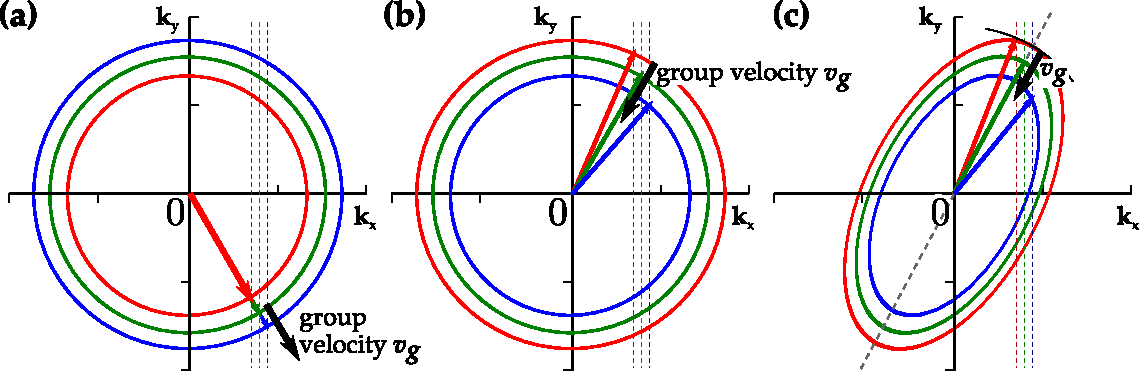
\includegraphics[width=.9\textwidth]{img/ifc_negrefr.pdf} 
\end{figure}
\begin{figure}[ht] \caption{Wavevector-dependent IFCs for one frequency, for the same medium as in Fig. \ref{fg_ifcnr} \todo{extend}} \label{fg_ifcnrk} \centering  %% TODO  WRITE
	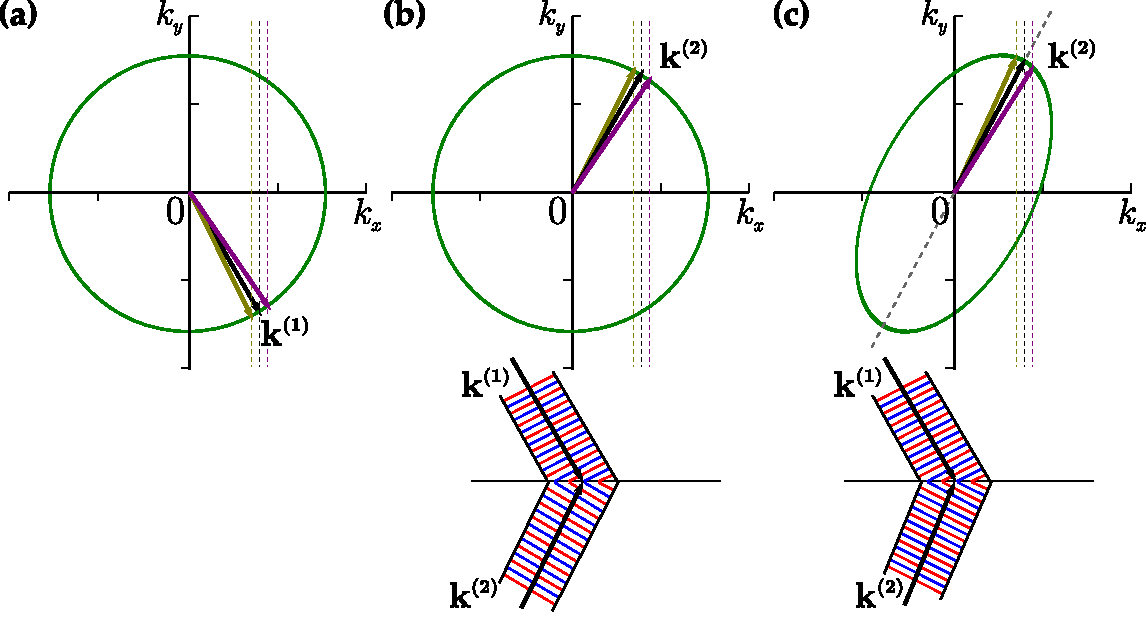
\includegraphics[width=.9\textwidth]{img/ifc_negrefrk.pdf} 
\end{figure}

Whenever the wave vector $\KK$ is nearly perpendicular to the isofrequency contour, which is the most often observed in isotropic media or in media where the wave vector points in a direction close to the optical axis, the Snell law is still applicable and we then speak of a \textit{negative index of refraction}.  The refraction between ordinary media and two examples involving negative-index media are plotted in Fig. \ref{fg_ifcnr}. It should be noted that the negative-index media always exhibity temporal dispersion. Therefore, the refraction of temporally short pulses disperses different frequencies into different angles, as can be seen from the wavevector orientation dependent on frequency in Fig. \ref{fg_ifcnr}b,c.
%% maybe?? the propagation velocities are more complicated 

%}}}

\section{Electrodynamics of nonlocal homogeneous media} 
\subsection{Nonlocal response} 
\paragraph{Definition of nonlocal media}%{{{
The previous two chapters that concerned local media can be generalized into the theory of \textit{nonlocal} (or, \textit{spatially dispersive}) media.  The downside of the spatial-dispersive model of media is that it is more complicated, leading e.g. to an implicit dispersion equation. Its great advantage is however that it provides a necessary level of generality for the description of periodic structures discussed below. 
Some phenomena observed in the frequency spectrum are in fact consequences of the spatial dispersion \cite[p. 359]{landau1984electrodynamics}, which is the case, for example, of the Doppler broadening of resonance lines in gases \cite{makarov2004permittivity}. 
These phenomena are primarily dependent on the wave vector $\kk$, and the apparent broadening on the \textit{frequency} axis is only due to the dispersion curve defining a simple relation between  frequency and wave vector.  

In this section, a general class of media is discussed, where the medium response explicitly depends on the history of $\E(\tau, \brho)$ in previous time $\tau < t$ and in all surrounding points $\brho$, and therefore it is described by a spatio-temporal convolution:
\begin{equation} \D(t,\rr) = \varepsilon_0 \E(t,\rr) + \varepsilon_0\int_{V} \int_{-\infty}^{t} \chi_e(t-\tau, \rr-\brho) \, \E(\tau,\brho) \,\mbox{d}\tau \,\mbox{d}^3\brho. \label{eq_chi_convol_nonloc}\end{equation}
In a very similar manner as in the local theory above, we assume that a plane wave $\E(t, \rr) := \E_0 \, e^{\ii\omega t - \ii\kk\cdot\rr}$ propagates through the medium. This is without loss of generality, since it is possible to express any wave as a superposition of monochromatic plane waves.
\begin{equation} \D(t,\rr) = \varepsilon_0 \E_0 \, e^{\ii\omega t - \ii\kk\cdot\rr} + \varepsilon_0\int_{V} \int_{-\infty}^{t} \chi_e(t-\tau, \rr-\brho) \, \E_0 \, e^{\ii\omega \tau - \ii\kk\cdot\brho} \,\mbox{d}\tau \,\mbox{d}^3\brho. \label{eq_chi_convol_harm_nonloc}\end{equation}
After two  substitutions, $T:=t-\tau$, $\mathbf{R}:=\rr-\brho$, the exponent can again be separated into the original plane wave (which factors out), and a spatio-temporal Fourier transform of the medium response:
$$				 \D(t,\rr) = \varepsilon_0 \E_0 \, e^{\ii\omega t - \ii\kk\cdot\rr} + \varepsilon_0\int_{V} \int_{-\infty}^{0} \chi_e(T, \mathbf{R}) \, \E_0 \, e^{\ii\omega (t - T) - \ii\kk\cdot(\rr - \mathbf{R})} \,\mbox{d}T \,\mbox{d}^3\brho,$$
$$				 \D(t,\rr) = \varepsilon_0 \E_0 \, e^{\ii\omega t - \ii\kk\cdot\rr} + \varepsilon_0\left( \int_{V} \int_{-\infty}^{0} \chi_e(T, \mathbf{R})  \, e^{-\ii\omega T + \ii\kk\cdot \mathbf{R}}\,\mbox{d}T \,\mbox{d}^3 \mathbf{R} \right) \E_0 \, e^{\ii\omega t - \ii\kk\cdot\rr}.$$
The response of the medium to the electric field of any harmonic plane wave can now be expressed as a function of frequency $\omega$ and wave vector $\kk$. It is defined as the ratio between the electric displacement and the electric field:
\begin{equation} \epsrn(\omega, \kk) = \left.\frac{\D(t,\rr)}{\varepsilon_0 \E(t,\rr)} \right|_{\E(t, \rr) := \E_0 \, e^{\ii\omega t - \ii\kk\cdot\rr}}  = 1 + \int_{V} \int_{-\infty}^{0} \chi_e(T, \mathbf{R}) \,e^{-\ii\omega T + \ii\kk\cdot \mathbf{R}} \,\mbox{d}T \,\mbox{d}^3\mathbf{R} \label{eq_eps_nonloc}\end{equation}
Converting the problem from the spatio-temporal domain into the wavenumber-frequency domain allows to express the relation between $\D$ and $\E$ by the \textit{permittivity} function $\epsrn(\omega, \kk)$ and completely avoid the convolution from Eq. (\ref{eq_chi_convol_harm_nonloc}). Note that both the response function $\chi_e$ and the permittivity $\epsrn$ 
may be either scalar functions, or rank-2 tensor functions; the latter case accounts for possible anisotropy of the medium.

The terms of \textit{nonlocality} and of \textit{spatial dispersion} are used interchangeably in the literature. The difference seems to be related to the way one thinks about the medium -- while \textit{nonlocality} is obviously related to the description in the real space [cf. Eq. (\ref{eq_chi_convol_nonloc})], \textit{spatial dispersion} derives from that the response is not a constant function in the reciprocal $\kk$-space. In the author's view, the term \textit{spatial dispersion} is therefore of a slightly narrower meaning, as it implies that an infinite plane wave of a defined wavevector is being considered.

%}}}
\paragraph{Power expansion of the medium parameters} %{{{
Assuming the permittivity $\epsrn(\omega,\kk)$ or permeability $\murn(\omega,\kk)$ are smooth functions varying slowly with $\kk$, we can express them in general as power series \cite[p. 367]{landau1984electrodynamics}:
\begin{equation} 
\left.  \begin{array}{c}
\epsrn(\omega,\kk) = 1 + \chi_e(\omega) + \ii \gamma_{\text{e}}(\omega) \kk + [\alpha_{\text{e}}(\omega) \kk] \kk + \ldots, \medskip  \\
\murn(\omega,\kk) = 1 + \chi_m(\omega) + \ii \gamma_{\text{m}}(\omega) \kk + [\alpha_{\text{m}}(\omega) \kk] \kk + \ldots, 
\end{array} \quad \right\} \quad \text{(in any media)}
\label{eq_epsmusd1}\end{equation} %% maybe change gamma->eta, alpha->phi, ...->psi, ...-xi ? 
where $\chi_{e,m}(\omega)$ are second rank tensors, $\gamma_{e,m}(\omega)$ third rank tensor, $\alpha_{e,m}(\omega)$ fourth rank, and similarly for possible higher orders of expansion. After the corresponding number of matrix multiplication with $\kk$, they all yield rank-2 tensors that add up to form the tensor of permittivity or permeability.
%In this customary symmetric approximation of local media, both the electric permittivity and permeability in Eq. (\ref{eq_eps_loc}) are composed of two terms, one caused by the immediate response of vacuum, and another by the response of matter. In nonlocal media, both functions depend on the wavevector $\kk$, making the solution of Maxwell equations more complicated.

Note the response function for a local medium can be formally derived from its nonlocal formulation by replacing the spatial dependence in Eq. (\ref{eq_chi_convol_nonloc}) by a Dirac delta function as follows: %% is the sencence correct?
\begin{equation} \chi_e(t-\tau, \rr-\brho) \rightarrow \delta^{3}(\rr-\brho) \; \chi_e(t-\tau), \label{eq_loc_chi}\end{equation}
which allows to simplify Eq. (\ref{eq_chi_convol_nonloc}) so that in local media only the temporal convolution has to be computed. Then the higher order terms including $\gamma_{e,m}$ and $\alpha_{e,m}$ in Eqs. (\ref{eq_epsmusd1}) vanish and
\begin{equation} 
\left.  \begin{array}{c}
\epsrn(\omega,\kk) = 1 + \chi_e(\omega) = \epsrl(\omega), \medskip \\
\murn(\omega,\kk) = 1 + \chi_m(\omega) = \murl(\omega). 
\end{array} \quad \right\} \quad \text{(in local media)}
\label{eq_epsmusd2}\end{equation}

%}}}
\paragraph{Magnetic effects can be described by nonlocal permittivity} %{{{
Here, we will follow the approach of Landau and Lifshitz (see \cite{landau1984electrodynamics}, and also \cite{krowne2007book_agran, agranovich2006spatial}) to show that the magnetic response of any medium can be fully expressed by a certain form of permittivity dependence on $\kk$. This leads to introducing new \textit{Landau-Lifshitz} permittivity $\epsLL$ and permeability $\muLL$, which are, in general, different from those used in the more customary symmetric model:
$$\epsLL(\omega, \kk) \not\equiv \epsrn(\omega, \kk),\quad\quad\quad 1 = \muLL(\omega, \kk) \not\equiv \murn(\omega, \kk).$$
The Maxwell equations (\ref{eq_me1}-\ref{eq_me4}) however still hold when these new parameters are substituted for the original ones. Requiring the relative permeability to be unity implies a trivial dependence of the magnetic field on the magnetic induction in this model:
$$ \mu_0 \HHsd = \B. $$

The advantage is that the relative magnetic permeability is defined as a mere constant of the magnetic response of vacuum $\muLL(\omega, \kk) := 1$, thus reducing the complexity of the computation compared to the symmetric spatial-dispersive model. %% [as in Eq. (\ref{eq_ce})]
Therefore, the \textit{Landau-Lifshitz} model developed below is also denoted as the $\E\D\B$-model, since it allows the substitution into the Maxwell equations to avoid explicit use of the magnetic field $\HH$.

%}}}
\paragraph{Local medium in the Landau-Lifshitz model} %{{{
An important step towards using the Landau-Lifshitz model is to explicitly derive how a classical, local medium with the magnetic response is represented. From the principle of correspondence, all local media can be expressed with this model without any change in the dispersion curves predicted. 

In the Landau-Lifshitz model, the new spatial-dispersive permittivity $\epsLL(\omega, \kk)$ consists of
\begin{enumerate}
 \item{the component caused by the local electric response of matter,} 
 \item{a new component fully accounting for the local \textit{magnetic} response of matter, thanks to a particular shape of its spatial dispersion.}
\end{enumerate}
Later, higher-order expansion terms can be easily added to describe all sorts of the nonlocal response.

Recalling the Maxwell equation (\ref{eq_me4}) that links the magnetic field $\HH$ with the electric induction $\D$, 
\begin{equation} \nabla \times \HH =  \frac{\partial \D} {\partial t}, \tag{\ref{eq_me4} \again} \end{equation}
it is clear that if one defines a new pair of vector fields
\begin{equation} \HHsd = \HH + \frac{\partial\mathbf{X}}{\partial t}, \label{eq_HHsd}\end{equation}
\begin{equation} \Dsd  = \D  + \nabla\times \mathbf{X}, \label{eq_Dsd}\end{equation}
then Eq. (\ref{eq_me4}) maintains exactly the same form with the new fields, for any differentiable vector field $\mathbf{X}$:
\begin{equation} \nabla \times \HHsd = \nabla \times \HH + \left(\nabla\times \frac{\partial\mathbf{X}}{\partial t}\right) = \frac{\partial \D}{\partial t}+ \frac{\partial(\nabla\times \mathbf{X})}{\partial t} =  \frac{\partial \Dsd} {\partial t}, \label{eq_me4sd} \end{equation}
because for reasonably shaped functions the temporal and spatial derivatives commute.

%% todo how this transform is denoted?
With the freedom of choice of $\mathbf{X}$, we impose the above mentioned requirement that whole magnetic response of the matter is expressed by the constitutive equation for permittivity. Therefore in spatial-dispersive theory, the constitutive equation 
for magnetic induction is defined the same as in vacuum, c.f. Eq. \ref{eq_ce}:
\begin{equation} \mu_0 \HHsd := \mu_0 \murl(\omega) \HH = \B. \label{eq_mu_sd}\end{equation}
When this equation is rearranged into the form similar to \ref{eq_HHsd}, we obtain a prescription for the sought $\mathbf{X}$: 
$$ \HHsd = \HH + (\murl(\omega) -1)\HH = \HH + \underbrace{\left(\frac{\murl(\omega)-1}{\mu_0\murl(\omega)}\right)\B}_{=:\,\partial\mathbf{X}/\partial t}$$
Without loss of generality, we again restrict the discussion to a plane wave (\ref{eq_pw}), thus the time derivative equals to multiplication by $\ii\omega$.
\begin{equation} \mathbf{X} = \frac{1}{\ii\omega}\left(\frac{\murl(\omega)-1}{\mu_0\murl(\omega)}\right)\B = \frac{1}{\ii\omega\mu_0}\left(1 - \frac{1}{\murl(\omega)}\right)\B. \label{eq_Xsd}\end{equation}
The new electric displacement $\Dsd$ in the  Landau-Lifshitz model, that also accounts for magnetic phenomena, is obtained by substitution of Eq. (\ref{eq_Xsd}) into Eq. (\ref{eq_Dsd}):
\begin{equation} \Dsd := \D - \ii\kk\times \mathbf{X} =  \D - \ii  \frac{1}{\ii\omega\mu_0}\left(1 - \frac{1}{\murl(\omega)}\right) \kk\times \B  \label{eq_Dsd2}\end{equation}
By means of the other Maxwell equation (\ref{eq_me3}), the magnetic induction $\B$ can be substituted by $\kk\times\E / \omega$ to obtain an expression that contains the electric quantities only.
\begin{equation} \Dsd = \D - \frac{1}{\omega^2 \mu_0}\left(1 - \frac{1}{\murl(\omega)}\right) \kk\times(\kk\times \E).  \label{eq_Dsd3}\end{equation} 
Double vector multiplication on the right hand side can be identified with the wave-plane projection tensor $\TT$, c.f. Eqs. (\ref{eq_rotrot}, \ref{eq_transverse1}):
\begin{equation} \Dsd = \D + \frac{k^2}{\omega^2 \mu_0}\left(1 - \frac{1}{\murl(\omega)}\right) \, \TT \E,  \label{eq_Dsd4}\end{equation} 

%}}}
\paragraph{Tensor form of the Landau-Lifshitz permittivity of local isotropic media}%{{{
%Continuing in the derivation outlined in , 
From Eq. (\ref{eq_Dsd3}) we can derive the tensor form of spatial-dispersive permittivity $\epsLL(\omega,\kk)$:
\begin{equation} 
\left.  \begin{array}{c}
\epsLL(\omega,\kk) = 1 \,+\, \chi_e(\omega) \;\;+\;\; \frac{k^2}{\omega^2 \mu_0}\left(1 - \frac{1}{\murl(\omega)}\right) \, \TT, \medskip \\
\muLL(\omega,\kk) = 1, 
\end{array} \quad \right\} \quad \text{(in local media)}
\label{eq_epsmusd3} \end{equation} 
where 
\begin{equation} \TT = \frac{1}{k^2} 
\left(\begin{array}{ccc} 
	k_y^2+k_z^2		& -k_x k_y		& -k_x k_z \\ 
	-k_y k_x		& k_x^2+k_z^2	& -k_y k_z \\ 
	-k_z k_x		& -k_z k_y		& k_x^2+k_y^2
	\end{array} \right) 
\text{ or equivalently, }
(\TT)_{ij} = - \frac{k_i k_j}{k^2} + \delta_{ij} . \tag{\ref{eq_transverse2} \again} \end{equation}

%}}}
\paragraph{Other formulations}%{{{
Let us note that the classical approach using symmetric parameters $\epsrl(\omega,\kk),\murl(\omega,\kk)$, and the Landau-Lifshitz approach of gathering all medium-related effects in the permittivity $\epsLL(\omega,\kk)$ are only two examples of all possible transformations of medium parameters that keep the Maxwell equations unchanged. 

Formally, it is possible to arbitrarily distribute the medium electric and magnetic responses between these parameters. The distribution weight may be even frequency dependent, leading to a physically realistic pair of parameters with custom spectral shape \cite{skaar2014diamagnetism}.
% maybe "Casimir" formulation of electrodynamics \cite{vinogradov2002form}
% TODO REF EBD theory and nonlocal electrodynamics %% \cite{krowne2007book_agran} %% \cite{landau1984electrodynamics} %% \cite{mikki2009electromagnetic}
%}}}

\subsection{Dispersion relations in nonlocal homogeneous media} 
\paragraph{Dispersion relation as an implicit equation} %{{{
In the dispersion relation for local media, Eq. (\ref{eq_dispdet}), the wave vector could be found by solving a set of linear equations. In the particular case of \textit{isotropic} local media, the computation has an even simpler form of an explicit computation of one square root, see Eq. (\ref{eq_dispeq_loc}).

An intrinsic issue of spatial-dispersive media is that the permittivity $\epsLL(\omega,\kk)$ is a function of the wavevector $\kk$ on its own. The dispersion equation then becomes an implicit equation similar to Eq. (\ref{eq_dispdet}), but now with $\epsLL$ dependent on $\kk$: 
\begin{equation} 
\det\left[
\TT -
	\frac{\mu_0 \varepsilon_0 \omega^2}{k^2}
	\left(\begin{array}{ccc} 
	{\epsLL}_{11}(\omega,\kk) & {\epsLL}_{21}(\omega,\kk) & {\epsLL}_{31}(\omega,\kk)  \\
	{\epsLL}_{12}(\omega,\kk) & {\epsLL}_{22}(\omega,\kk) & {\epsLL}_{32}(\omega,\kk)  \\
	{\epsLL}_{13}(\omega,\kk) & {\epsLL}_{23}(\omega,\kk) & {\epsLL}_{33}(\omega,\kk)  
	\end{array} \right) \right] = 0. \label{eq_dispdetLL}\end{equation}
If all tensor elements, ${\epsLL}_{ij}(\omega,\kk)$, can be approximated in the form of a polynomial expansion to a low order in $\kk$, the solution can again be found as roots of a characteristic polynomial. The degree of this polynomial may be substantially higher than in Eq. (\ref{eq_dispdet}), the dispersion curves can nonetheless be found by a brutal-force numerical search. %% ?? for any ${\epsLL}_{ij}(\omega,\kk)$.
\begin{figure}[t] \caption{Dispersion curves for three different types of local media, comparing the local and Landau-Lifshitz representations of constitutive parameters. Three rows show media with \textbf{(a)} a  resonance in permittivity, \textbf{(b)} in permeability, and \textbf{(c)} in both parameters simultaneously.\\
Left column: Local parameters $\epsrl(\omega)$, $\murl(\omega)$ as functions of frequency. Right column: Dispersion curves were computed either with the local parameters from Eq. (\ref{eq_epsmusd2}) [plotted as green lines] or with the Landau-Lifshitz parameters from Eq. (\ref{eq_epsmusd3}) [plotted as black contour]. The Landau-Lifshitz permittivity $\epsLL(\omega,\kk)$ is color shaded on the background.
} \label{fg_dcll} \centering  
\textbf{(a)}\\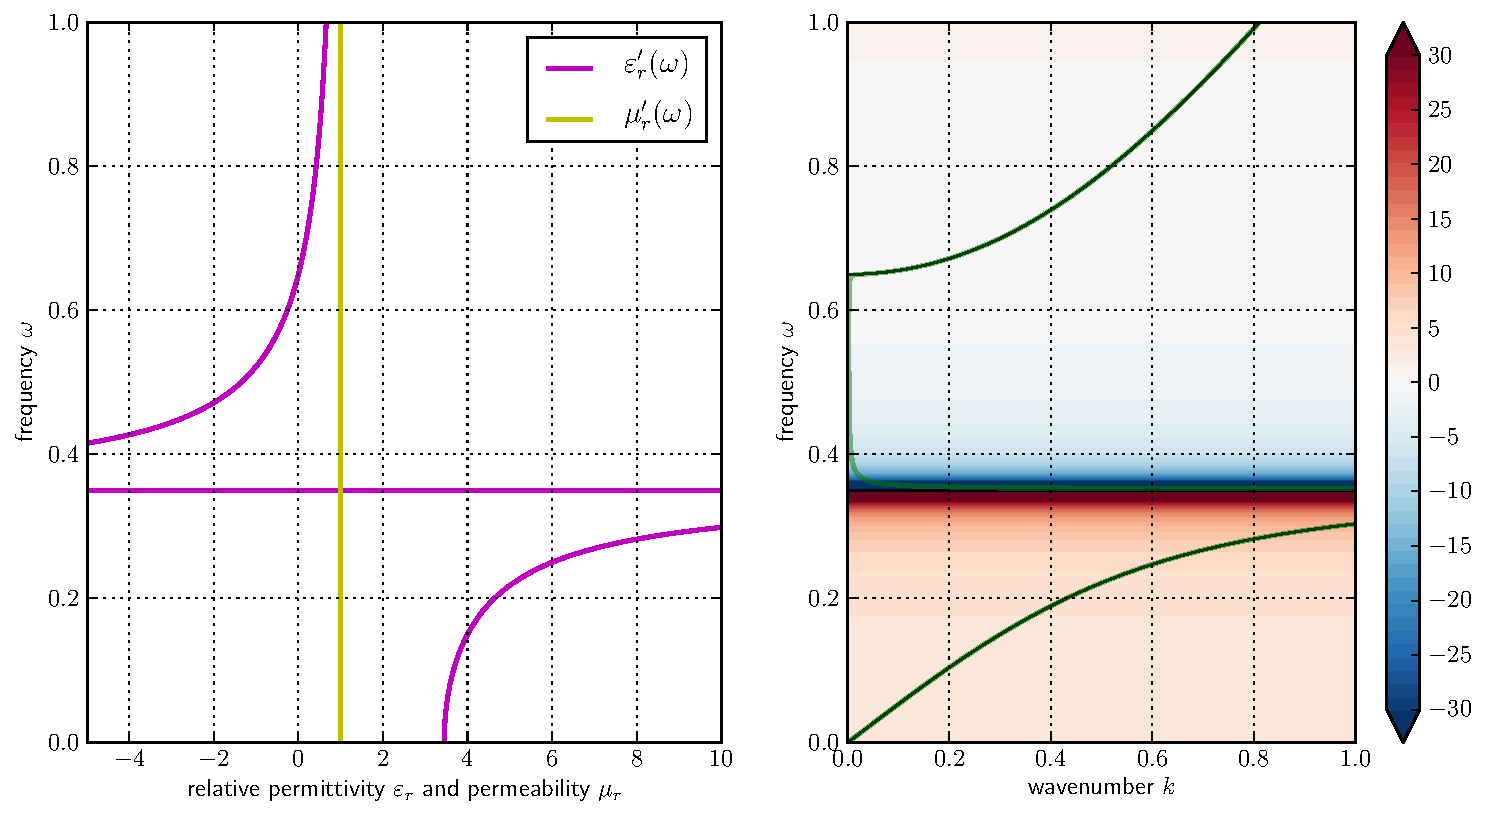
\includegraphics[width=1\textwidth]{img/dispersion_landau_lifshitz/dispersion_ll_el.pdf}    
\textbf{(b)}\\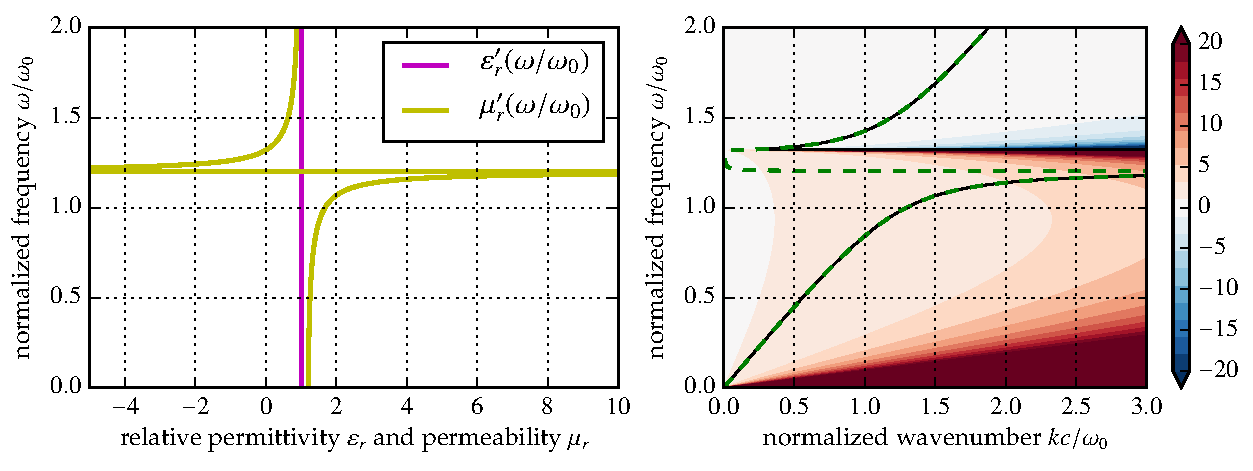
\includegraphics[width=1\textwidth]{img/dispersion_landau_lifshitz/dispersion_ll_mag.pdf}
\textbf{(c)}\\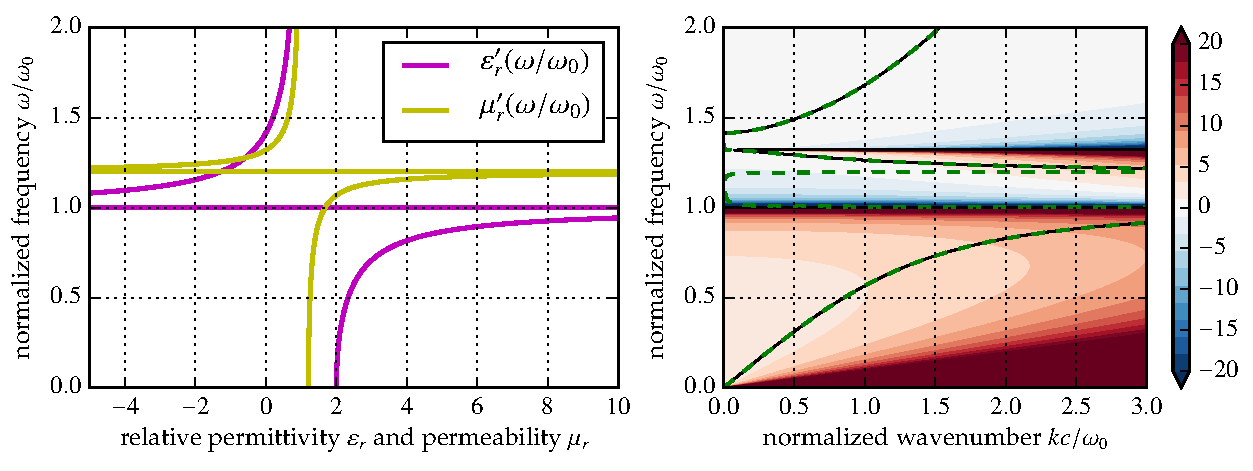
\includegraphics[width=1\textwidth]{img/dispersion_landau_lifshitz/dispersion_ll_elmag.pdf}
\end{figure}
\clearpage

%}}}
\paragraph{Dispersion of a local dielectric in the Landau-Lifshitz model} %{{{
The dispersion curves predicted by the classical and Landau-Lifshitz representations of the constitutive parameters for local media in Eq. (\ref{eq_epsmusd3}) are mathematically identical. This is illustrated by Fig. \ref{fg_dcll} on three examples: of a medium with (\ref{fg_dcll}a) an electric resonance, with (\ref{fg_dcll}b) a magnetic resonance and (\ref{fg_dcll}c) with both resonances overlapping. 

The plots in the left column of Fig. \ref{fg_dcll} show the \textit{local} permittivity $\epsrl(\omega)$ and permeability $\murl(\omega)$.
Its right column features a thin black contour connecting all points where the dispersion equation (\ref{eq_dispdetLL}) was found to hold by a numerical search.
This is complemented by the Landau-Lifshitz permittivity $\epsLL(\omega, k)$ as a background colour map with blue tone for negative values and red for positive ones. 
%As a confirmation of the compatibility of the Landau-Lifshitz model with the classical one,
Additionally, the original green dispersion curve as in Fig. \ref{fg_dcsimpleel} is retained, as computed using the classical approach based on the Eq. (\ref{eq_dispeq_loc}). It can thus be seen that both models always predict exactly the same dispersion.

For a local isotropic medium with a single electric resonance in Fig. \ref{fg_dcll}a, the curves plotted are identical to Fig. \ref{fg_dcsimpleel}. On the right panel, the Landau-Lifshitz permittivity $\epsLL(\omega, k)$ follows a resonance curve in frequency, but is independent of the wavenumber $k$ (as long as the medium is local). With frequency increasing, the lower polariton branch bends towards higher $k$, as $\epsLL(\omega, k)$ increases towards the resonance at $\omega_0$, then a band of frequency follows where and no solution of the wave equation %% TODO REF
exists due to $\epsLL(\omega, k)$ being negative, and finally the upper polariton branch starts when $\epsLL(\omega, k)$ crosses zero and becomes positive again.

A local medium with a single \textit{magnetic} resonance, Fig. \ref{fg_dcll}b, is predicted by the symmetric model to exhibit similar dispersion curves. In the right panel of Fig. \ref{fg_dcll}b, the magnetic resonance is represented by the
contribution that grows proportionally with $k^2$: 
\begin{equation} \Dsd = \D + \underbrace{\frac{k^2}{\omega^2 \mu_0}\left(1 - \frac{1}{\murl(\omega)}\right) \, \TT \E}_{\text{magnetic contribution}},      \tag{\ref{eq_Dsd4} \again} \end{equation}
% TODO FK: Nějak to tam nevidím. To jako pro ω/ω0> 1.3? Chtělo by to popsat nějak názorněji.
and unlike the case of the electric resonance, the maximum magnitude of the magnetic contribution is located at the frequency $\omega_{mp}$ where $\murl(\omega_{mp}) \rightarrow 0$. In the plot \ref{fg_dcll}b, this is at $\omega/\omega_0 \approx 1.3$.
% TODO FK: Ani tady se mi nezdá zjevné, kde je tato podmínka splněna.
This shape of $\epsLL(\omega, k)$ causes the lower polariton branch to bend and approach a horizontal asymptote, which is again separated by a band of no allowed wave from the upper polariton branch, starting at $\omega_{mp}$.
$\epsLL(\omega, k)$

Finally, in Fig. \ref{fg_dcll}c, both resonances are combined. The main difference from the cases of isolated resonances occurs in the frequency range where originally $\epsLL(\omega, k) < 0$ and no wave could propagate. However, the magnetic resonance increases $\epsLL(\omega, k)$ by a term proportional to $k^2$, and consequently a new photonic branch is formed with $\mathrm{d}\omega/\mathrm{d}k < 0$, that is, with opposite group and phase velocities. IFCs for the new band then appear as sketched in Figs. \ref{fg_ifcnr}b and \ref{fg_ifcnrk}b.
% (electric quadrupoles..., [Merlin])
% todo Why magnetic resonances do not contribute to the static permeability?

%% XXX up to here revision of FK 2015-06-28 XXX

%}}}
\paragraph{The dispersion of nonlocal media} %{{{ 
\begin{figure}[t] \caption{Dispersion curves for two nonlocal media. They differ by the value of the fourth-order expansion coefficient $\alpha(\omega)$, which was plotted with a thin blue line. The left and right columns of plots show the same information as in Fig. \ref{fg_dcll}.  } \label{fg_dcll_nl} \centering  
\textbf{(a)}\\	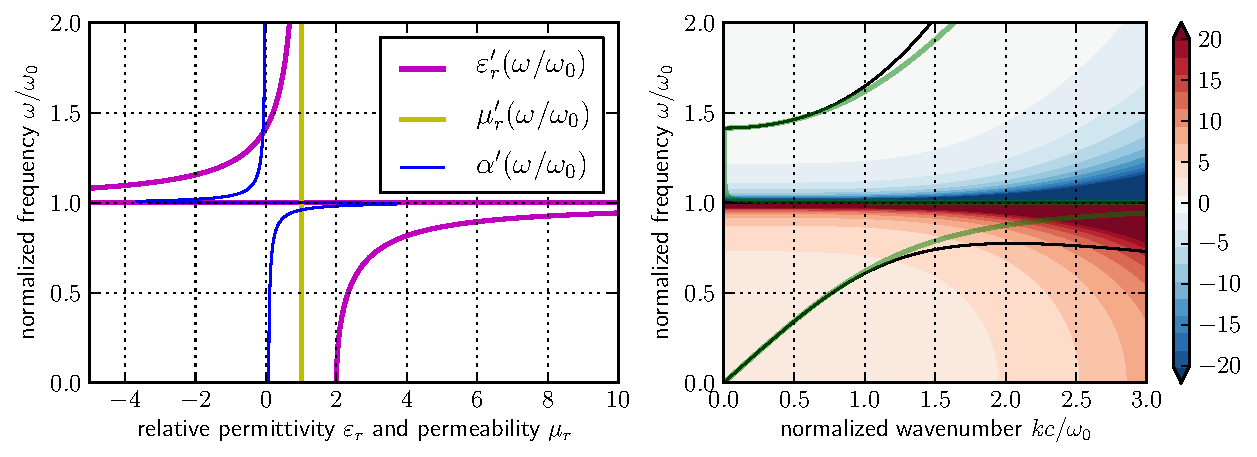
\includegraphics[width=1\textwidth]{img/dispersion_landau_lifshitz/dispersion_ll_quadrupp.pdf}
\textbf{(b)}\\	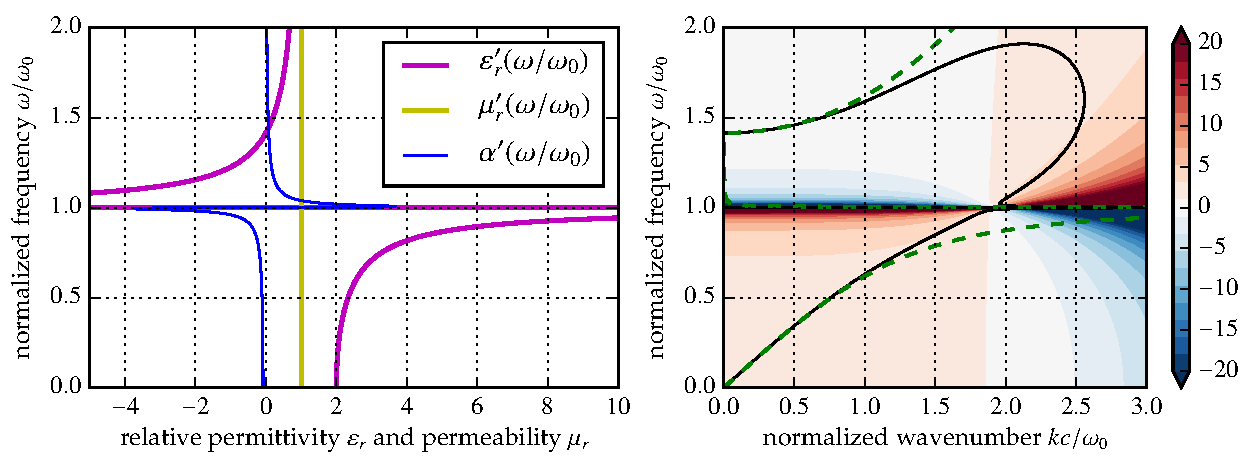
\includegraphics[width=1\textwidth]{img/dispersion_landau_lifshitz/dispersion_ll_quadrupn.pdf}
\end{figure}
Further terms in the permittivity $\epsLL(\omega,\kk)$ expansion in Eq. \ref{eq_epsmusd3} lead the dispersion curves to deviate from those predicted for local media. This corresponds to the black contour deviating from the green line in Fig. \ref{fg_dcll_nl}.
As the simplest example we add one scalar term $\alpha(\omega) k^4$ to $\epsLL(\omega,\kk)$ in Eq. (\ref{eq_epsmusd1}). The shape of $\alpha(\omega)$  was chosen as a weak Lorentz oscillator at the resonance frequency of the ordinary electric response $\chi_e(\omega)$. This is reflected in adding a thin blue line in the left column.

\label{chap_sd}
The choice of using the same resonance frequency for $\chi_e(\omega)$ and $\alpha(\omega)$ is not arbitrary; it is assumed that both terms arise from the same resonance mode that has field shape different from that of a simple dipole. The relation of higher-order expansion terms of Landau-Lifshitz permittivity  to the multipole expansion of the field shape is developed e.g. in Refs. \cite{agranovich2006spatial}, \cite{vinogradov2002form} and \cite{fietz2011homogenization}.

The choices of positive amplitude (Fig. \ref{fg_dcll_nl}a) and a negative one (Fig. \ref{fg_dcll_nl}b) have characteristic impacts on the dispersion curves. In the former case, both polariton branches deviate away from each other with frequency growing. In the latter case, they come closer to each other with growing $k$. Eventually, in the upper right corner of the right plot in Fig. \ref{fg_dcll_nl}b, they merge into one loop. Author however believes this merging may not be observed in nature, and that its occurrence is only due to unrealistic values of the $\alpha(\omega)$ coefficient, and absence of higher-order expansion terms.

%}}}
\paragraph{Multiple waves and additional boundary conditions}   %{{{ 
For both cases shown in Fig. \ref{fg_dcll_nl}, it follows that the dispersion equations can allow multiple solutions with different wavenumber $k$ at one frequency $\omega$, even when the waves have the same orientation and polarisation. (Note that, conversely, multiple solutions with different $\omega$ for a given wavevector $\kk$ are commonly present, as a usual consequence of frequency dispersion even in local media.)

The waves propagating with the higher wavenumber $k$ are denoted as \textit{additional} waves, were predicted by the works of Pekar and others
%\cite{agranovich2006spatial, agranovich2004linear, krowne2007book, agranovich1962crystal}
and also suggested by experimental data of dispersion near exciton levels e.g. in cadmium sulphide
\cite{pekar1975spatial}. 

In the case of a positive amplitude of $\alpha$ (c.f. Fig. \ref{fg_dcll_nl}a), one of the two solutions of the lower polariton branch has opposite signs of the wavevector and the group velocity ($|\vg| = \mathrm{d}\omega/\mathrm{d}k < 0$), giving raise to negative index of refraction in natural homogeneous media.

%}}}
\paragraph{Odd expansion terms and optical activity }   %{{{ 
Returning to the power expansion of $\epsLL(\omega, \kk)$ in terms of $k$ in Eq. (\ref{eq_epsmusd1}), we can identify the term constant in $k$ with the electric dipole moment $\chi_e(\omega)$, the term proportional to $k^2$ with the magnetic dipole moment $\chi_m(\omega)$ (or, also the electric quadrupole moment), and the recently discussed term proportional to $k^4$ with an electric octupole or magnetic quadrupole (\cite{agranovich2006spatial, agranovich2004linear, krowne2007book}).

The odd expansion terms were not discussed yet, although they have important physical interpretation -- their nonzero values break the spatial inversion symmetry of the medium, and are thus related to optical activity \cite{bungay1993equivalency}. 
In media with nonzero odd terms, the corresponding eigenwaves are circularly polarized, and they propagate with different velocity, feeling opposite signs of the odd expansion terms. Thus, the two plots in the right column of Fig. \ref{fg_dcllactivity} can also be viewed as the dispersion curves of the same medium, for the left and right circularly polarized waves.

\begin{figure}[t] \caption{Dispersion curves for two media with optical activity. The left and right columns of plots show the same information as in Figs. \ref{fg_dcll} and \ref{fg_dcll_nl}. The frequency dependence of the function $\gamma_e(\omega)$, which occurs in the term linearly proportional to $k$ in the expansion (\ref{eq_epsmusd1}), is plotted in the left column as a thin red line. } \label{fg_dcllactivity} \centering  
\textbf{(a)}\\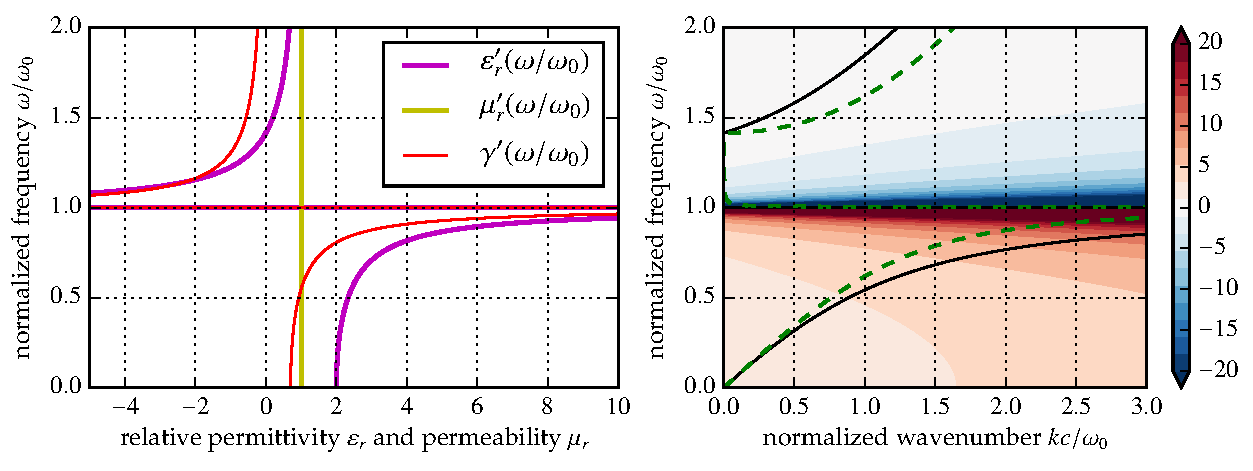
\includegraphics[width=1\textwidth]{img/dispersion_landau_lifshitz/dispersion_ll_activep.pdf}
\textbf{(b)}\\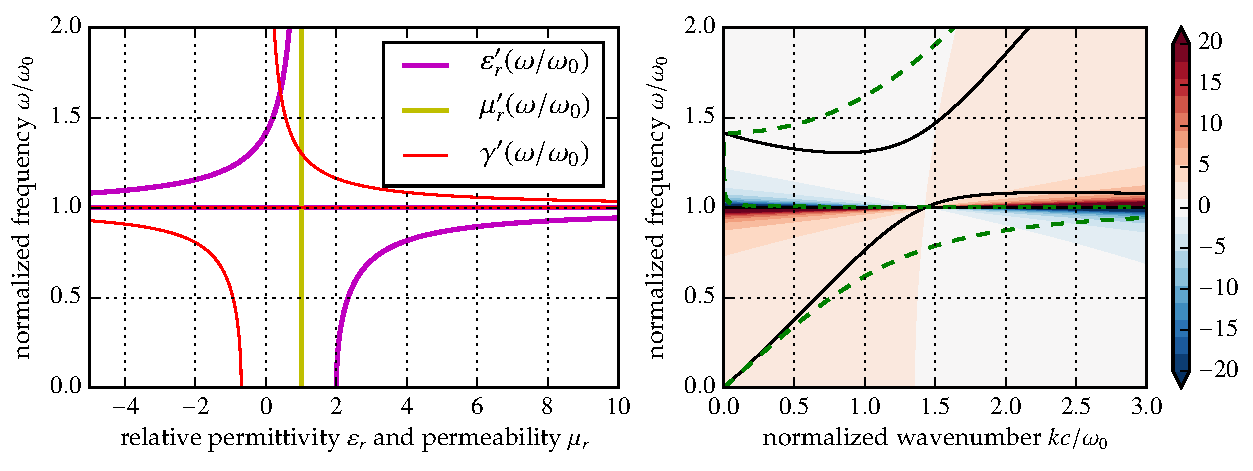
\includegraphics[width=1\textwidth]{img/dispersion_landau_lifshitz/dispersion_ll_activen.pdf}
\end{figure}

%}}}

\subsection{Amplitudes of the refraction and reflection}
\paragraph{The interface of two local media} %{{{ 
In the previous text, only the phase-related phenomena were discussed and the dependence of the dispersion curves and IFCs was computed as a result of the local or nonlocal response of the medium. Geometrical arguments then were used to infer the angle of refraction at the interface of two media, showing e.g. that a positive or negative refraction may occur, that the beam may refract in a different direction than the wave vector, and that in some cases the notion of index of refraction can be used to simplify the problem to a mere substitution into the Snell law.

The conservation of the wave phase at the interface is, however, not the only constraint to the refraction and reflection problem. Assuming there is no surface current nor surface charge, and that both media are local, the \textit{parallel} component of the fields $\E$, $\HH$ with regards to the interface must be continuous. Additionally, the \textit{perpendicular} component of the displacements $\D$, $\B$ is continuous, too. This rule can be deduced from the Maxwell equations [Eq.  (\ref{eq_me1}--\ref{eq_me4})], integrating them over infinitesimally thin loops or surfaces, respectively, that are symmetrically placed on the interface \cite[pp. 26-29]{klingshirn2007semiconductor}. 

The reflection and refraction (i.e. transmission) coefficients for the \textit{amplitudes} of the waves are derived in many textbooks  with different levels of generalisation.  
In the particular case where wave perpendicularly impinges the interface of two isotropic local media, described by their \textit{impedances} $Z_1, Z_2$, respectively, the (complex) reflection $r$ and transmission $t$ are
\begin{equation} r = \frac{Z_2 - Z_1}{Z_2+Z_1}, \quad t = \frac{2 Z_2}{Z_2 + Z_1}, \label{eq_reflection}\end{equation}
with the impedance of each medium
$Z_{1} = \sqrt{\frac{\murl}{\epsrl}}$.
Eq. (\ref{eq_reflection}) is analogous to the reflection on a one-dimensional transmission line, as known from the microwave engineering, although the impedance of a transmission line is defined in a more complicated way than in a continuous medium.
The complex amplitudes of the reflected and transmitted wave depend on the angle of incidence, and splits into the TE and TM polarisation \cite[p. 38]{born1999book}.  % todo add analytic eqs.?

%}}}
\paragraph{Refraction on interface with a nonlocal medium}   %{{{ TODO
To compute the amplitudes of reflection and transmission for nonlocal media is a substantially more complicated task than for the local media. The fundamental reason is related to that the definition of the medium response (\ref{eq_chi_convol_nonloc}) contains a convolution over an infinite space, which naturally does not account for the interface. For the problem to be better formulated, the integral would have to be modified, either with the nonlocal response of medium to extend also behind the interface, or with the medium response sharply truncated at the interface.

For weak spatial dispersion, different approaches to the problem are discussed (and corrected) in \cite{golubkov1995boundary}. %Extending the notion of impedance to spatial-dispersive media to compute the amplitudes. 

%}}}

\subsection{Phase, group, energy and signal velocity}
\paragraph{Signs of the phase and group velocities}%{{{ TODO
The negative refraction in media shown in Figs. \ref{fg_ifcnr}b,c and \ref{fg_ifcnrk}b,c was a result of the requirement for the group velocity $\vg$ to maintain its component perpendicular to the interface, and for the wave vector $\kk$ to maintain its projection onto the plane of interface. 

It was assumed that the group velocity coincides with the energy or information propagation, and therefore that it should always be "positive", that is, it should propagate towards the interface in the first medium and outwards from it in the second one.  in the following paragraphs, This assumption will be challenged for special cases, but usually it is correct and the terminology of \textit{negative phase} velocity is used when it is opposite to the group velocity.

Therefore, in media with low losses, the term of negative refraction 

\add{... in media with time reversal, the wave may always propagate backwards - we should always speak of mutual sign of the velocities}

phase velocity is often higher than the speed of light, this is no problem\\

%}}}
\paragraph{Signs of the group and energy velocities}  % TODO %{{{
%  \mdf{
%  % TODO 0401 how can one tell apart negative refraction due to eps-mu and due to higher, purely nonlocal terms?
%  *doubly resonant local media -> negative phase velocity, positive group velocity, above resonant frequencies - theoretically arbitrarily small losses\\
%  *singly resonant local media -> positive phase velocity, negative group velocity, this happens near resonance so there are always high losses\\
%  *			  nonlocal media -> weird things happen, todo\\
%  }
In the discussion of wave refraction on an interface, it was assumed that the envelope (or modulation) of the wave approaches the interface in the first medium, then refracts and propagates out \textit{from} the interface in the second medium. The envelope propagates with the group velocity, $\vg$, as defined by Eq. (\ref{eq_vg}). There is another quantity, the \textit{Poynting vector} $\mathbf{P} := \E\times\HH$, describing the direction and density of the \textit{power} carried by the optical wave. \todo{cite}

The group velocity usually points in the same direction as the Poynting vector, but this has not necessarily to be always true. A typical counterexample can be found near resonances in lossy (local) media. Such a behaviour can be traced back to Fig. \ref{fg_oscillator_spectrum}, where the permittivity drops from high values to negative ones. If the medium is defined as a lossy one, the curve of the wavenumber $k(\omega)$ is continuous and smooth, and as a result the magnitude of the group velocity $v_g = \mathrm{d}\omega / \mathrm{d}k$ is negative around the resonance for $\omega \sim 2\pi$, %% TODO "negative" means "opposite to kk"? But we are speaking of scalars...
which is also known as \textit{anomalous dispersion}. 

It follows from this that the group velocity $\vg$ can also point opposite to the Poynting vector that represents propagation of the light beam energy, $\mathbf{S}$. 
% This fact can not be easily deduced from the dispersion curves or IFCs. %% TODO  Or can it?
This behaviour can be observed in narrow parts of the spectrum only, around the resonance frequencies where the media have high losses, and also a strong group velocity dispersion.
Assuming passivity and absence of sources in the second medium, it is obviously the Poynting vector that has to maintain its perpendicular component and that the group velocity has inevitably to point towards the interface also in the second medium, which seems contradictory to causality.
This result 
%of the light envelope propagating with the group velocity \textit{from} the second medium \textit{towards} the interface may seem unphysical, 
may however be explained through strong deformation of the envelope shape on a short distance, which ensures the information carried by the wave modulation to propagate causally, out from the source, and always with speed lower or equal to the speed of light in vacuum $c$.

Negative group velocity has been experimentally observed in a thin sample. It manifested as a negative shift of the light envelope compared to the absence of the medium \cite{dolling2006simultaneous}. Note that the negative group velocity is independent of the sign of the phase velocity, which may be both positive and negative \cite{mikki2009electromagnetic}.

%}}}
\paragraph{Signal velocity}%{{{
The notion of \textit{signal} or \textit{information propagation velocity} is sometimes % TODO cite
identified with the group velocity, $\vg$. However, this may be misleading, as the differential definition of the group velocity in Eq. (\ref{eq_vg}) enables one to define it for slow-enough modulation only, so that the span of frequencies is narrow and the second derivative, corresponding to the group velocity dispersion, can be neglected.

Assuming the information is carried by a wave modulation that is limited in time (e. g. presence or absence of an optical pulse), one leaves the comfortable approximation of narrow spectrum: from the convolution-multiplication theorem already used in Eq. (\ref{eq_kkresult}), it can be shown that any information carrying function with a compact support has to span over an infinite spectrum. The proof \cite{hill2013uncertainty} can be drawn along the line of that under multiplication by some compact-supported binary functions, e.g., 
$$ f(t) \rightarrow f(t) \cdot \mathrm{sign}^2[f(t)], $$
the original function does not change.

A temporally limited optical pulse will be always more or less distorted upon propagation in dispersive medium where the dispersion curves are not straight. Then the information velocity becomes a problematic term. If the information can be detected exactly in the first moment when the fields deviate from strict zero, one comes to the surprising conclusion that, in dispersive media, the information propagates probably with the speed of light. In the opposite example of a highly noisy channel, the pulse may be reliably detected only after most its energy already arrived. To conclude, the author is convinced that the notion of \textit{information velocity} is too vague unless its exact definition is provided first, and should not be directly associated with the group velocity. 

%}}}
%% TODO \paragraph{Speed of light and causality in nonlocal media}%{{{
%% \mdf{TODO REF Kramers-Kronig relations in nonlocal medium
%% \cite{skettrup1970kramers}
%% \cite{kirzhnitz1976}
%% \cite{melrose1977generalised}
%% \cite{sun1989kramers}
%% \cite{rozanov2003}
%% \cite{bruleanalysis}
%% \cite{makarov2013kramers}
%% }%}}}

\section{Electromagnetic waves in periodic structures}
\subsection{Periodic structures and the Bloch theorem}
\paragraph{Inhomogeneity}%{{{
The previous sections discussed infinite media, with the only deviation from homogenity at an interface of two media, where refraction of the waves is observed, and it was shown that the resulting orientation of the wave vector and of the group velocity could be easily deduced on geometrical basis. The amplitude of the reflected and refracted waves can be also easily computed for local media, whereas their computation for nonlocal media is much less straightforward. 

There is a broader class of structures for which analytical or semianalytical methods have been developed to compute their interaction with electromagnetic waves, such as scattering on dielectric/metallic spheres, propagation through arbitrary stacks of parallel layers, diffraction on thin apertures, resonances in orthogonal, cylindrical or spherical cavities, or wave guiding in high-symmetry waveguides or optical fibers. 

The interaction of electromagnetic waves with most of possible structures is too complex to be expressed analytically, and can only be accessed by numerical methods, some of which are described in Chapter \ref{chapter_numerical}. However, when these elementary structures are arranged into an infinite array, the resulting periodic structure behaves in a way that is characteristic for the periodicity and its most important traits can again be partially understood on analytical basis.
This chapter focuses on these general properties shared by periodic structures, leaving the particular numerical simulations to the Results section.

%}}}
\paragraph{Periodicity}%{{{
Under the notion of \textit{periodicity} we understand there exist discrete translational symmetries. In three dimensions, that is 
\begin{equation} \epsrl(\omega,\rr) = \epsrl(\rr + m_1 \ava + m_2 \avb + m_3 \avc) \quad\text{ where }\quad m_1, m_2, m_3 \in \mathbb{Z} \label{eq_trsym}\end{equation}
and $\ava, \avb, \avc$ are three linearly independent vectors. The permittivity, given by Eq. (\ref{eq_lorentz_eps}), was intuitively generalized to a function of the position $\rr$. The same periodicity is also imposed on the permeability $\murl(\omega,\rr)$ and possibly all other quantities. Note that the constituent media are described by the \textit{local} quantities only, to avoid possible problems at the boundary computing the spatial convolution  in nonlocal media, Eq. (\ref{eq_eps_nonloc}). 

The points generated by all combinations of possible translations by $m_1 \ava + m_2 \avb + m_3 \avc$ form a periodic lattice.
The volume defined as a \textit{set of points closest to} one given point of the lattice will be denoted as a \textit{unit cell} (similar to the \textit{Wigner-Seitz cell} in solid-state physics). Obviously, the permittivity or permeability in periodic structures needs only to be specified in the domain of one unit cell.

The choice of lattice vectors $\avabc$ limits the set of the rotation or mirror symmetries of the structure. Based on the allowed symmetries, all lattices in three dimensions can be classified into six \textit{crystal families}, namely \textit{cubic}, \textit{tetragonal}, \textit{ortorhombic}, \textit{monoclinic}, \textit{hexagonal-trigonal} and \textit{triclinic}. Combined with additional restrictions of the symmetry given by the structure with each unit cell, all periodic structures can be classified into total 230 \textit{crystallographic point groups}. Numerous crystal optics textbooks (e.g. \cite[p. 678]{born1999book}) give more rigorous definitions. 

Unless stated otherwise, we will assume that the cubic lattice is used, which allows the highest possible symmetry. In the cubic lattice, the lattice vectors $\avabc$ are of the same magnitude $a$ and mutually orthogonal. % Note, however, that even the structure with a periodic modulation of permittivity is no more isotropic, i.e. posessing continuous rotational symmetry.

%}}}
\paragraph{The Bloch theorem}%{{{
The \textit{Bloch} (or \textit{Bloch-Floquet}) theorem states that while the harmonic wave is no more a solution for the Maxwell equations in a periodic structure that conforms to Eq. (\ref{eq_trsym}), a solution can always be found as a \textit{Bloch wave} -- a product of a harmonic function and another periodic one:
\begin{equation} 
\E(t, \rr) = \mathbf{u_e}(\rr)\,\mathrm{e}^{\ii\omega t - \ii\KK\cdot\rr}, \text{ where } \mathbf{u_e}(\rr) = \mathbf{u_e}(\rr + m_1 \ava + m_2 \avc + m_3 \avc),
\label{eq_bloch}\end{equation} 
\begin{equation}
\HH(t, \rr) = \mathbf{u_m}(\rr)\,\mathrm{e}^{\ii\omega t - \ii\KK\cdot\rr}, \text{ where } \mathbf{u_m}(\rr) = \mathbf{u_m}(\rr + m_1 \ava + m_2 \avb + m_3 \avc).
\label{eq_blochh}\end{equation} 
As a rule of all linear systems, any sum of Bloch waves is also a proper solution, but for simplicity we will focus on one Bloch wave at a time.

Functions $\mathbf{u_e}(\rr)$ and $\mathbf{u_m}(\rr)$ have the same periodicity as the structure, and will be denoted as the \textit{mode functions}. They are, in general, complex vector functions, so they not only alter the direction and magnitude of the electric and magnetic fields, but can also introduce a \textit{phase modulation} of the wave in each unit cell. 

The remaining term, $e^{\ii\omega t - \ii\KK\cdot\rr}$, is analogous to that of a plane wave
\begin{equation} \E(t, \rr) := \E_0\, e^{\ii\omega t - \ii\kk\cdot\rr}, \tag{\ref{eq_pw} \again} \end{equation}
except for the capital $\KK$ being used to distinguish the wave vector of the Bloch wave envelope from the wave vector $\kk$ in homogeneous media. 

Note that the Bloch theorem does not determine the shape of $\mathbf{u_e}(\rr)$, $\mathbf{u_m}(\rr)$, nor the direction and magnitude of $\KK$, it only states a solution in the form of Eqs. (\ref{eq_bloch}, \ref{eq_blochh}) can be found.
% TODO proof /home/filip/PhD/Sources_MM_theory/Bloch_Theorem_Proof.pdf
% TODO example illustration of Bloch wave -> plotted in Python

%}}}
\paragraph{Proof of the Bloch theorem}%{{{
This theorem is essential for understanding the electromagnetic behaviour of periodic structures, and it deserves a proof. Originally, it was developed for the electron wave function $\psi$ in crystals on the basis of quantum mechanics. The outline of such a proof in one dimension, which is the most often found in textbooks (e.g. \cite[p. 134]{ashcroft2005solid}) is based on the following:
\label{blochproof}
\begin{enumerate}
 \item{We assume $\psi$ is an eigenfunction of the Hamiltonian: $\exists h\in \mathbb{C}: \hat H\psi = h\psi$.} 
 \item{We also assume that the Hamiltonian operator $\hat H$ commutes with the operator of discrete translation $\hat T$ by the inter-atomic distance: $\forall \psi: \hat H\hat T\psi = \hat T\hat H\psi$. } 
 \item{Then $(T\psi)$ is an eigenfunction of $H$, because obviously $\hat H(\hat T\psi) \stackrel{1.}{=} \hat T\hat H\psi \stackrel{2.}{=} \hat Th\psi = h(\hat T\psi)$. \todo{this is perhaps redundant; remove this step?} }
 \item{From two eigenfunction relations, $\hat H\psi\stackrel{2.}{=} h\psi$ and $\hat H(\hat T\psi) \stackrel{3.}{=} h(\hat T\psi)$, it also follows that $\psi$ is eigenfunction of the translation operator, that is,
$\exists K\in \mathbb{C}: \hat T\psi = e^{-\ii Ka}\psi$. \todo{HT=TH implies eig common} Therefore, the eigenfunction $\psi$ is unchanged upon a discrete translation, differing only by the phase being shifted by $-Ka$. Setting $a$ to be the unit cell size, $K$ becomes the wavenumber of the Bloch wave envelope.
%$\exists t\in \mathbb{C}: hT\psi = HT\psi = Ht\psi = ht\psi$. \todo{cite} %In the special case that more eigenfunctions are associated 
}
 \end{enumerate}
Two commuting operators share the same eigenstates, which means that the electron wave function at a given energy (i.e. Hamiltonian eigenfunction) must also have a discrete translational symmetry provided its phase can change between atoms (i.e. it is an eigenfunction of the non-hermitian translation operator).

%}}}
\paragraph{The proof in the electromagnetic formulation}%{{{
The steps can be reformulated replacing the abstract Hamiltonian with an operator derived from the Maxwell equations. In a periodic structure one can no longer assume the solution in the form of a plane wave (\ref{eq_pw}), but as long as the structure is time-invariant and linear, the monochromatic electric and magnetic fields can still be decomposed into a product of some complex function of space position, and a harmonic function of time:
\begin{equation} 
\begin{array}{cc}
\E(t, \rr) = \E(\rr) e^{\ii \omega t}, \\
\HH(t, \rr) = \HH(\rr) e^{\ii \omega t}. 
\end{array}
\label{eq_harmonic}\end{equation}
One thus only needs to prove the Bloch theorem for the time-invariant parts of the fields, which will play the same role as the wavefunction $\psi$ in the quantum-mechanical formulation.

\begin{enumerate}
\item{
For $\E(\rr)$ to be a  valid solution of Maxwell equations in the periodic structure at the angular frequency $\omega$,
it can be derived from Eq. (\ref{eq_me3}, \ref{eq_me4}, \ref{eq_epstensor} and \ref{eq_harmonic}) in straightforward manner that
\begin{equation} 
{\epsrl}^{-1}(\omega,\rr) \nabla\times \left[{\murl}^{-1 }(\omega,\rr) \nabla\times \E(\rr) \right] = \frac{\omega^2}{c^2}\E(\rr).   \label{eq_eigen_e}
\end{equation}
In analogy with the quantum-mechanical proof, the left hand side of Eq. (\ref{eq_eigen_e}) can be associated with the Hamiltonian $\hat H\psi$, and the right hand side with its eigenvalue $h\psi$ \cite{johnson2003introduction}. 
} 
\item{
The translation operator acts by substitution of the position vector $\rr$ in the argument. For example, the translated electric field is
\begin{equation} \hat T\psi \rightarrow \E(\rr+\mathbf{a_1}). \label{eq_blocht}\end{equation}
The commutation relation directly follows from the periodicity in Eq. (\ref{eq_trsym}), thus the right terms in Eqs. (\ref{eq_blochht}) and (\ref{eq_blochth}) are identical by definition:
\begin{equation} \hat H \hat T \psi \quad  \rightarrow \quad  {\epsrl}^{-1}(\omega,\rr    ) \nabla\times \left[{\murl}^{-1 }(\omega,\rr    ) \nabla\times \E(\rr+\ava)\right]  \label{eq_blochht}\end{equation}
\begin{equation} \hat T \hat H \psi \quad  \rightarrow \quad  {\epsrl}^{-1}(\omega,\rr+\ava) \nabla\times \left[{\murl}^{-1 }(\omega,\rr+\ava) \nabla\times \E(\rr+\ava)\right] .  \label{eq_blochth}\end{equation}
In three dimensions, this argument is valid for three different translation operators that correspond to the addition of the different lattice vectors, $\ava$, $\avb$ and $\avc$.
} 
\item{
Then the wave translated by any of the lattice vectors, is also a solution of the Maxwell equations:
\begin{equation}  {\epsrl}^{-1}(\omega,\rr) \nabla\times \left[{\murl}^{-1 }(\omega,\rr) \nabla\times   \E(\rr+\ava)\right] =  \frac{\omega^2}{c^2}\E(\rr+\ava).  \label{eq_blochme}\end{equation}
}
\item{In analogy with the fourth step in the Bloch theorem proof, there exists at least one constant $K_1$ for which
\begin{equation}  \E(\rr+\ava) = e^{-\ii K_1 a_1} \E(\rr),  \label{eq_blochtt}\end{equation}
	where $K_1 a_1$ represents the phase shift between the adjacent cells along the direction of the lattice vector $\ava$. In a similar manner, constants $K_2$ and $K_3$ can be associated with the translation by the $\avb$ and $\avc$ vectors, respectively. 
}
 \end{enumerate}

%}}}
\paragraph{Bloch theorem in three dimensions} %{{{
The three constants $K_{1,2,3}$ then define the \textit{Bloch wave vector} $\KK$: \todo{expand, and refer to symbols above}
\begin{equation} \KK := 
\frac{2\pi K_1(\avb\times\avc)}{\ava\cdot(\avb\times\avc)} +  
\frac{2\pi K_2(\avc\times\ava)}{\avb\cdot(\avc\times\ava)} +  
\frac{2\pi K_3(\ava\times\avb)}{\avc\cdot(\ava\times\avb)}.
\label{eq_reciprocalK}\end{equation}
If the lattice vectors $\avabc$ are orthogonal, Eq. (\ref{eq_reciprocalK}) simplifies to
% $K_{1,2,3}$ directly define the projection of the $\KK$:
\begin{equation} \KK := 
	\frac{2\pi K_1 \ava}{a_1^{2}} +  
	\frac{2\pi K_2 \avb}{a_2^{2}} +  
	\frac{2\pi K_3 \avc}{a_3^{2}}.
\label{eq_reciprocalKorto}\end{equation}

Repeating the procedure for the magnetic field, a similar operator can be obtained, where the multiplication by ${\epsrl}^{-1}(\omega,\rr)$ and ${\murl}^{-1 }(\omega,\rr)$ occurs in the opposite order. Thus the same arguments, with the identical wave vector $\KK$, have to be valid also for the magnetic field $\HH(\rr)$, where the Hamiltonian is associated with an operator very similar to that of the electric field in Eq. (\ref{eq_eigen_e}):
\begin{equation}
{\murl}^{-1 }(\omega,\rr) \nabla\times \left[{\epsrl}^{-1}(\omega,\rr) \nabla\times \HH(\rr)\right] = \frac{\omega^2}{c^2}\HH(\rr).   \label{eq_eigen_h}
\end{equation}

%}}}
\paragraph{Virtual periodicity and ambiguity of the mode function}%{{{
Homogeneous media, such as vacuum, naturally fulfill the definition of periodicity in Eq. (\ref{eq_trsym}).
From the principle of correspondence, the Bloch theorem must predict
the already known solution of a harmonic plane wave in vacuum
\begin{equation} \E(t, \rr) := \E_0\, e^{\ii\omega t - \ii\kk\cdot\rr}. \tag{\ref{eq_pw} \again} \end{equation}
The expected solution of the Bloch wave in vacuum can be directly found as a formal modification of the dispersion relation,
\begin{equation}  
\E(t, \rr) = \mathbf{u_e}(\rr)\,\mathrm{e}^{\ii\omega t - \ii\KK\cdot\rr}, \text{ where } \mathbf{u_e}(\rr) := \E_0  \text{ and } \KK := \kk.
\label{eq_blochvac}
\end{equation}
However, this is not the only possible representation of a plane wave as the Bloch wave, as the Eqs. (\ref{eq_bloch}, \ref{eq_blochh}) are mathematically ambiguous. 
For illustration, using the fact that any lattice of periodic unit cells may be imagined in vacuum, one can choose a cubic lattice with an arbitrary unit cell size $a$, % TODO represent by lattice vectors G?
for which the plane wave in vacuum can be simultaneously represented by any of infinitely many other combinations of
\begin{equation} 
\left.  \begin{array}{cc}
	\mathbf{u_{e}}(\rr) := \E_0 e^{2\pi\ii (m_1\ava\cdot\rr + m_2/\avb\cdot\rr + m_3/\avc\cdot\rr)/a^{2}} \vspace{2mm} \\ %% TODO use mathbf here? or is this whole a rubbish?
%\KK := \kk - \frac{2\pi m_1}{a_1} - \frac{2\pi m_2}{a_2}- \frac{2\pi m_3}{a_3},
\end{array}\quad \right\} \quad \forall m_{1,2,3} \in \mathbb{Z}
\label{eq_blochvac2}
\end{equation}
%\begin{equation} \KK := 
	%\frac{2\pi K_1 \mathbf{a_1}}{a_1^{2}} +  
	%\frac{2\pi K_2 \mathbf{a_2}}{a_2^{2}} +  
	%\frac{2\pi K_3 \mathbf{a_3}}{a_3^{2}}.
%\label{eq_reciprocalKorto}\end{equation}
which all 
%maintain the requirement of the mode function $\mathbf{u_{e}}(\rr)$ being periodic and still 
give the exactly same resulting plane wave. 

\begin{figure}[ht] \caption{Folded and unfolded dispersion curves for free space and a periodic structure viewed along one of its axes. The phase difference over a unit cell can be expressed either by the wavenumber $K$ (unfolded plots \textbf{a, b} above), or it can be partially absorbed into the periodic mode function $\mathbf{u}(\rr)$ (folded plots \textbf{c, d} below)\\
The lattice periodicity allows to draw the dispersion curves of periodic structures using natural scale-invariant units, with the Bloch wave number $K$ divided by the spatial frequency of the lattice $2\pi/a$, and the angular frequency $\omega$ multiplied by the time needed for the light to traverse the unit cell.
} \label{fg_phcfolding} \centering  %% TODO write caption; complement the text to match
	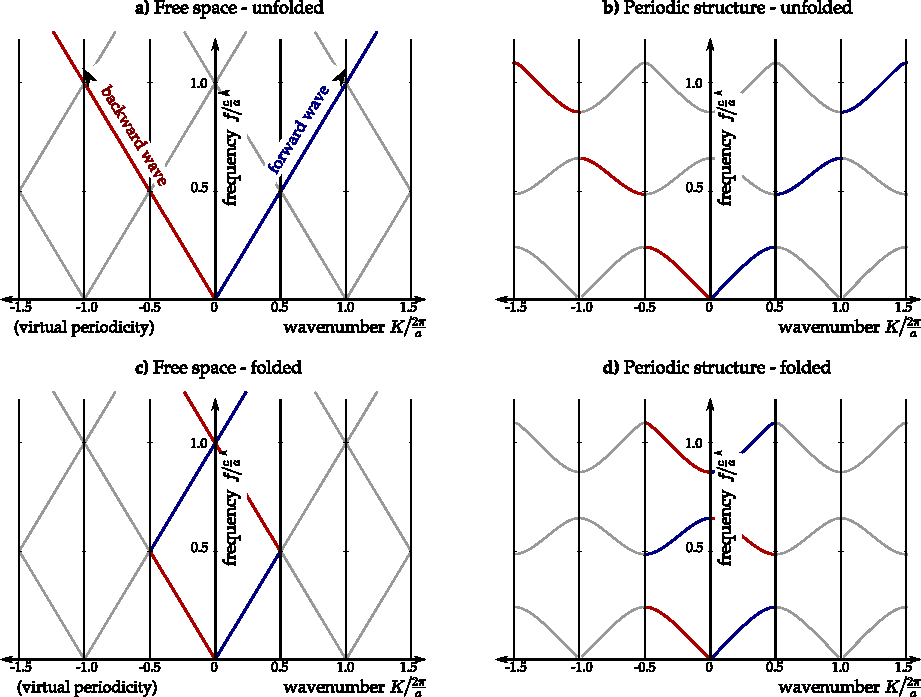
\includegraphics[width=\textwidth]{img/PhC_folding_illustration.pdf} 
\end{figure}
\clearpage

%}}}

\subsection{Dispersion in periodic structures}
\paragraph{Folding of the dispersion curves} %{{{
All possible dispersion curves for a \textit{Bloch wave in vacuum} with the $\KK$ vector oriented along one lattice axis in vacuum are plotted in Fig. \ref{fg_phcfolding}a. The dispersion curve for the original forward wave from Eq. (\ref{eq_blochvac}) is plotted in blue; another solution exists for a wave propagating in the opposite direction which is plotted in red. All other solutions generated by Eq. (\ref{eq_blochvac2}) are plotted in gray, for both forward and backward waves. 
Note that the actual physical shape of the fields in space,  $\E(\rr)$ and $\HH(\rr)$, can not be deduced from the dispersion curve. To fully determine the fields, the dispersion curves would have to be complemented by the mode functions $\mathbf{u_e}(\rr)$ and $\mathbf{u_m}(\rr)$ (that depend on the frequency). 

\label{par_disp_curv_per}
The inherent ambiguity of description on the basis of the Bloch wave can be used to graphically save space in the plot by showing the dispersion curves only for $K\in\langle-\pi/a, \pi/a\rangle$, as shown in Fig. \ref{fg_phcfolding}c. Plotting any other interval of equal width would be equivalent \cite[p. 177]{brillouin2003wave}. 

The space of the plot can be further halved, since all forward and backward propagating solutions are symmetrical with respect to the vertical $K=0$ axis, except for structures with optical activity (c.f. Fig. \ref{fg_dcllactivity}) or even breaking the time-reversal symmetry (c.f. Ref. \cite{vanwolleghem2009unidirectional}), which are not discussed in this thesis. Thus, in many papers on periodic structures, all dispersion curves are plotted as \textit{folded} in the $K\in\langle0, \pi/a\rangle$ region only \cite{obrien2002photonic,yannopapas2005negative}. In some other references, such as \cite{mortensen2010unambiguous} or \cite{yeh1977electromagnetic}, unfolded dispersion curves are used.

The mathematical interpretation of folding the dispersion curves in vacuum can be found from Eq. (\ref{eq_blochvac2}): 
\begin{enumerate}
\item{
For  $\omega\in\langle 0, \pi c /a\rangle$, the mode function is constant in space, $\mathbf{u_e}(\rr) := E_0$, and $K := \omega/c$. 
} 
\item{
At the first point of folding for $K=\pi/a$, the mode function changes to $\mathbf{u_e}(\rr) := E_0 e^{2\pi\ii r/a}$ and the formal solution of the \textit{backward} wave is used with $K := 2\pi r/a - \omega r/c$.  The phase advance across one unit cell remains positive, since the negative phase advance of the backward-wave envelope is less than the phase contribution of the mode function.
} 
\item{
When the dispersion curve touches the $K=0$ axis at the frequency $\omega = 2\pi c/a$, the mode function is not changed, but the dispersion curve continues again along with the \textit{forward} wave $K := - 2\pi r/a + \omega r/c$. 
} 
 \end{enumerate}
In vacuum, this process repeats with higher orders of the mode function: $\mathbf{u_e}(\rr) := E_0 e^{4\pi\ii r/a}$, $\mathbf{u_e}(\rr) := E_0 e^{6\pi\ii r/a}$, etc.

We will show in the Results section on a particular example that some numerical approaches provide nontrivial rules to prefer one particular dispersion curve in the unfolded plot. The Results section also contains a physical interpretation of this.

%When the wavelength is less than double cell spacing, or equivalently when $2\pi c /K < 2 a$, the unit cells can scatter the forward propagating wave into the backward direction and vice versa. In an infinite periodic structure the energy transfer must be conserved, so the forward and backward waves must be of the same amplitude. (The equilibrium of forward and backward wave amplitudes may, however, differ in some cases even in in infinite periodic structure. One example is when the constituent materials lose time-reversal symmetry due to static magnetic field.) We assume this also in this example with virtual periodicity. The \textit{Bloch wave} is a product of two functions, and it gives one degree of freedom to select which part of (\ref{eq_bloch}) expresses the phase shift across one unit cell. Two different conventions are used in the literature.
% \begin{enumerate}
%  \item{In the \textit{unfolded} plot, the phase shift is expressed entirely by the envelope $\mathrm{e}^{\mathrm{i}Kz}$. One can always find a line coming from the front side of a unit cell to its back side, along which the mode function does not change its phase significantly $\mathbf{u(\mathbf{r})}$. In other words, the volume of the unit cell is not divided by any \textit{nodal plane} in the real part of electric field  $\mathbf{u(\mathbf{r})}$. (However, closed nodal planes within the unit cell may appear due to individual resonances.)
% 
% In vacuum, the mode function takes the simplest form, being constant $\mathbf{u(\rr)} = 1$ at all frequencies. The dispersion relation of vacuum forms a direct line as plotted in Fig. \ref{fg_phcfolding}a.} 
%  \item{The \textit{folded} plot requires $K/\left(\frac{2\pi}{a}\right) \in (-\frac{1}{2}, \frac{1}{2})$ and the remaining phase is mostly expressed by the mode function. 
% Further savings of space in the plot can be made using the symmetry of the forward and backward waves, so only the positive half for $K/\left(\frac{2\pi}{a}\right) \in (0, \frac{1}{2})$ has to be plotted to describe the mode structure.} 
% \end{enumerate}
% Although maybe less instructive, usually the \textit{folded} bands are plotted in the literature and they are used also in Fig. \ref{fg_1dbd}, \ref{fg_rodh} and \ref{fg_erod_radius11} below. The same approach can be used for periodic structures, where the bands are separated by band gaps, cf. Fig. \ref{fg_phcfolding}b and \ref{fg_phcfolding}d.

%}}}
\paragraph{Fourier expansion of the mode function}%{{{ 
If the periodic structure is not homogeneous, that is, $\epsrl(\omega,\rr)$ or $\murl(\omega,\rr)$ depends on $\rr$, the mode functions $\mathbf{u_{em}}(\rr)$ are no more constant nor harmonic as they were in Eq. (\ref{eq_blochvac2}). They however still share the periodicity of the lattice, as dictated by the Bloch theorem in Eq. (\ref{eq_bloch}), and their exact shape can thus be decomposed into Fourier series
characteristic for the structure and the frequency of operation, defining nonzero amplitudes for all branches. The grey lines plotted in Fig. \ref{fg_phcfolding} then are no more hypothetical solutions to be chosen from, but they all have real amplitudes, and are present simultaneously. 
Note this does not contradict the ambiguity of choice of the Bloch wavevector $\KK$, which stems from the  mathematical representation of the Bloch wave.

%}}}
\paragraph{Brillouin zones in the reciprocal space} %{{{ 
The periodically repeated one-dimensional interval of $K\in\langle-\pi/a, \pi/a\rangle$ can be viewed as the unit cell in the space of wave vectors, i.e. in the \textit{reciprocal space}. This unit cell is then denoted as the first \textit{Brillouin zone}.  \todo{unify somehow the alternating explanation in 1-D and 3-D}
The $m$-th Brillouin zone is defined as the set of all points for which the center point $K=0$ is the $m$-th closest point in the lattice. 
All Brillouin zones have equal measure, and moreover, they can be rearranged into the first one by simple translation. %% TODO specify what this re-arrangement means

In the one-dimensional case the definition of higher Brillouin zones trivially consists in dividing the axis symetrically into equal intervals, such as $K\in\langle-2\pi/a, -\pi/a\rangle \cup \langle \pi/a, 2\pi/a\rangle$ for the second one etc. 

In two or three dimensions the shapes of higher Brillouin zones become much more complex, and are unlike to each other \cite[pp. 134--135]{klingshirn2007semiconductor}: in two dimensions, all Brillouin zones are composed of polygons that are connected in their vertices to encircle the previous Brillouin zone \cite[p. 126]{brillouin2003wave}. Similarly, in three dimensions, they are composed of polyhedra connected by their edges, and their shape roughly resembles sphere shells. 

The above illustration of how the plot space can be spared by folding the dispersion curves into the first Brillouin zone also applies to two- or three-dimensional structures.
%, where it actually becomes a practical help for visualisation. TODO rm this?
The exact shapes of the Brillouin zones are determined by the \textit{crystal family} of the real-space lattice and its set of lattice vectors $\avabc$. 
As was also noted above, the space occupied by the plot can be further reduced thanks to the symmetry of the dispersion curves. This naturally applies to higher dimensions as well; the minimum part of the Brillouin zone that contains all necessary information is denoted as the \textit{irreducible Brillouin zone} and is determined by the crystallographic point group of the lattice. 

More detailed listing and comparison of Brillouin zone shapes is beyond the scope of this thesis, but can be found in numerous solid-state textbooks, e.g. \cite[pp. 96-99]{klingshirn2007semiconductor}. %% TODO add some good detailed textbook on BZ

%}}}
\paragraph{High-symmetry points of the Brillouin zones} %{{{ 
The fundamental difference between plotting of one dispersion curve and the isofrequency contours (IFCs) is that IFCs give the information about the dispersion for a two-dimensional scan of the wave vector $\KK$, whereas the dispersion curve is limited to only a one-dimensional scan along some line in the $\KK$-space (c.f. Fig. \ref{fg_ifc_dc}). The limitation is even more significant in the case of three dimensions, where it is virtually impossible to visualize the frequency $\omega(\KK)$ as a function of three components of $\KK$.

A hybrid approach can be taken, however, that maintains most of the physical information about the dispersion in the two- or three-dimensional structures. It consists in plotting the  dispersion curves around the boundary or edges of one selected irreducible Brillouin zone. It is expected that no important information is lost by leaving out its inner surface.

The notation of high-symmetry points in the $\KK$-space is standardized. For the square lattice in two dimensions, four high-symmetry points are named as follows: "$\mathbf{\Gamma}$" corresponds to the center, $K=0$. Provided that the first lattice vector $\ava$ is parallel to the $x$-axis of the coordinate system, the point where $\KK = (\pi/a, 0)$ is denoted as  "$\mathbf{X}$" and the point $\KK = (0, \pi/a)$ as "$\mathbf{Y}$". Finally, the diagonal point of $\KK = (\pi/a, \pi/a)$ is known as "$\mathbf{M}$".
In two-dimensional case, the dispersion curves are typically plotted along the triangle encircling the irreducible Brillouin zone: $\mathbf{\Gamma}-\mathbf{X}-\mathbf{M}-\mathbf{\Gamma}$.

In three-dimensional cubic lattice, these points maintain their meaning in the plane perpendicular to the $z$-axis \cite[p. 99]{klingshirn2007semiconductor}. Additionally, "$\mathbf{R}$" denotes the spatial diagonal of $\KK = (\pi/a, \pi/a, \pi/a)$. Other lattices introduce more complex sets of the high-symmetry points and the paths along which the dispersion curves are plotted do not seem to be standardized.

\todo{Figure - irr Brill zone for square and cubic lattices}

\todo{Figure - Gamma-X-K-Gamma dc}

%}}}
%% \paragraph{Dispersion curves for the reduced Brillouin zone} %{{{ 
%% %}}}
\paragraph{Tight-binding model for the photonic band-gaps} %{{{
The notation of the high-symmetry points in the Brillouin zone can outline a different way of understanding the origin of the dispersion, which can be drawn in analogy with the \textit{tight-binding},   %% TODO cite?
or also \textit{hopping},  %% TODO cite?
model in solid-state physics. 

\label{tight-binding}
Analyzing one unit cell isolated in free space, one obtains its natural resonance frequency.  When the cell is surrounded by other cells in the periodic lattice, their mutual coupling alters the resonance frequency \cite[p. 75]{klingshirn2007semiconductor}; the actual sign of the coupling effect does not seem to be determined by any simple general rule, however.	

For a steady oscillatory solution to be obtained, the electromagnetic fields in the surrounding cells must have the same modulus of oscillation amplitude, but they do not need to share the phase. This is equivalent to a single Bloch wave propagating in the structure. 

Identical phase in all cells corresponds to zero Bloch wave vector, $\KK = 0$, and to the point $\mathbf{\Gamma}$ in the center of the Brillouin zone. Under the basic assumption that the fields $\E, \HH$ are continuous and smooth vector functions, identical phase of adjacent cells translates into
\begin{equation} \frac{\partial \E}{\partial\mathbf{n}} = \frac{\partial \HH}{\partial\mathbf{n}} = 0 \quad\text{(Neumann boundary conditions).} \label{eq_bcond_neumann}\end{equation} 
Here, the operator $\partial/\partial \mathbf{n}$ denotes the derivative along the normal to the boundaries.

Other special cases are observed when $\KK$ is in some of the high-symmetry points of the Brillouin zone. For the simple case of a two-dimensional square lattice, the $\mathbf{M}$-point corresponds to the adjacent cells having exactly opposite phase of the fields. This requires that the field amplitudes at the boundary are zero:
\begin{equation} \E = \HH = 0 \quad\text{(Dirichlet boundary conditions).} \label{eq_bcond_dirichlet}\end{equation} 

The $\mathbf{X}$ and $\mathbf{Y}$ points are combination of the Dirichlet and Neumann boundary conditions for two different directions.
As a generalization of the above mentioned, the boundary conditions can be found for any point in the Brillouin zone, provided that correct phase difference between all opposite faces is correctly maintained.

The stronger the coupling between the neighbouring cells, the bigger the difference between the resonance frequencies for the $\mathbf{\Gamma}$ and $\mathbf{X}$ points. Returning to the definition of the group velocity in Eq. (\ref{eq_vg}), one comes to the already expected fact that the energy transfer is proportional to the strength of the inter-cell coupling.

%}}}
%%% \paragraph{Spatial dispersion in photonic structures} %{{{  TODO develop
%%% Near the $\mathbf{\Gamma}$, $\mathbf{\Gamma}$K~or $\mathbf{\Gamma}$M points, the spatial dispersion must be strong to account for the zero group velocity, and actual bending of the dispersion curve downwards in the adjacent zone. The effect can however not be directly interpreted as the negative group velocity, as the dispersion curve only corresponds to one term in the Fourier expansion of the field shape. 
%%% %}}}

\subsection{Band-gaps} 
\paragraph{Properties of band-gaps} %{{{
In the plots of dispersion curves, one could identify ranges of frequencies which were not associated with any dispersion curve. 
They could be observed for a local dielectric (Figs. \ref{fg_dcsimpleel} and \ref{fg_dcll}), for nonlocal dielectrics (Figs. \ref{fg_dcll_nl}, \ref{fg_dcllactivity}), as well as for periodic structures in Fig. \ref{fg_phcfolding}. Such regions are denoted as (electromagnetic) \textit{band-gaps}. They are a very common phenomenon both in dispersive homogeneous media and periodic structures. 
While the wave propagation received due attention in the above, also the wave "non-propagation" deserves to be commented here.
%It is essential to point out the similarities and eventual differences between them.

The band-gap behaviour is simplest to describe in isotropic media, analogous to the one-dimensional case: for a frequency within the band-gap, no wavevector $\KK$ can be found under which the electromagnetic wave would propagate, or more precisely, there is no real wavevector for which the (Bloch) wave would be a solution of Maxwell equations. In the more complicated cases of a harmonic plane wave in anisotropic homogeneous media, or of a Bloch wave in any periodic structure, the band-gap properties depend on the field polarisation and on the direction under which the wave propagates. Many such media, for example, exhibit a band-gap for one polarisation and only in some set of wave vector orientations.

A familiar scenario is that a wave propagates through a transparent medium (e.g. glass) and impinges an interface with a band-gap medium (e.g. metal). In the latter, it is not allowed to propagate, and all its energy reflects back into the first medium. The Maxwell equations however require that the fields do not end abruptly at the interface; in particular, it follows from the linearity of the medium that the \textit{evanescent} wave amplitude decays in the second medium in an exponential manner with the distance below the interface.

If losses are present, part of the impinging wave energy may be also dissipated. Nonetheless, he exponential decay of the evanescent wave should not be confused with the exponential nature of the Lambert-Beer law in absorbing media.

A scenario less typical, but not less instructive, is when a dipole source is embedded in the infinite medium and is forced by some external mechanism to oscillate at some frequency within the band-gap. Intuitively, one could expect such a "hard" dipole will inevitably put energy into the medium. In reality, the effect of the medium surrounding the dipole will make the dipole act, with regards the driving force, as a purely elastic or inertial load. In particular, if the dipole is realized as an antenna driven by a high-frequency circuit, it will appear to the circuit as purely capacitive or inductive load. Thus, for continuous oscillations, all energy will be returned to the driving mechanism. 

To prevent the energy from being returned to the source, one can further imagine the energy is pushed into the dipole in a very short pulse, and then the dipole completely disappears. However, the nature of the band-gap can not be overcome: from the convolution-multiplication theorem, such a pulsed source would have a broad spectrum and it would radiate the energy in the neighbouring allowed bands. 

% }}}
\paragraph{Band-gaps stemming from individual resonances}%{{{
One common class of band-gaps is based on \textit{individual resonances} in the medium or structure. These band-gaps are often observed in realistic natural media, where the resonances arise from the vibration of electrons, atoms or molecules, as described above. 
Although realistic media are composed of a lattice of individual atoms, which would suggest that even here the wave has the Bloch form of Eqs. (\ref{eq_bloch},\ref{eq_blochh}), the atoms are roughly $10^{4}$ times smaller than the wavelength, and the electromagnetic wave can be sufficiently approximated as a harmonic wave in Eq. (\ref{eq_pw}) with a well-defined wavelength.  To make this harmonic approximation, it is important that these particles are small and close to each other compared to the wavelength. % ; otherwise  % 

Periodic structures can similarly exhibit a resonance confined in the unit cell. 
To the author's knowledge,  %% XX?
every possible shape formed from a dielectric or metal has infinitely many resonance modes,  %% ... high-permittivity and...
characteristic by relatively high concentration of energy in the structure, or near to it, and relatively weak coupling to the incident electromagnetic wave.  %% ... More specific rules will be given in the Results.
Arranging such resonant elements into the lattice is a fundamental step in building a periodic structure with resonant behaviour. In such structures, the dispersion for the Bloch wave follows a resonance curve similar (but not the same) as in Fig. \ref{fg_oscillator_spectrum}. Sometimes the behaviour of the Bloch wave is described as \textit{macroscopic}, while the fields localized in the resonant elements as \textit{mesoscopic} \cite{felbacq2005theory}, and the word \textit{microscopic} is left for the much finer fields in the constituent atoms or molecules.

Another important characteristic of individual resonances is in a \textit{qualitative} change in the field shape between the lower and upper edge of the band-gap. This is true for natural media as well as for lattices of individual resonators. Typically, at the lower band-gap edge, the dipoles are \textit{in-phase} with the wave, whereas at the upper edge, they are \textit{in counter-phase}.  % TODO note also that these indiv resonances are typical by a resonance shape in the permitivity
Inside the bandgap, usually closer to the lower frequency edge, a resonance frequency is located (c.f. Fig. \ref{fg_oscillator_spectrum}).

Yet another characteristic is that the resonant interaction of a particle with the wave can be approximated as a point dipole or multipole. As is dictated by the symmetry of the resonant field in the particle, the dipole moment may be electric, magnetic, zero or both simultaneously. A particle has multiple resonances at different frequencies, each of them having usually either an electric or a magnetic dipole. In particles of lower symmetry, one resonant mode may have both nonzero dipole moments simultaneously; this leads to optical activity. 

Other resonances have both dipole moments zero, which in general results from higher rotational symmetry of the fields. Their interaction with the electromagnetic wave is mediated by the electric or magnetic \textit{quadrupole moment} (or even higher \textit{multipole} \cite{merlin2009metamaterials}). This interaction is usually weak, however it grows with the wavenumber $k$. Such multipole moments often complement dipole resonances, and are responsible for spatial dispersion, see Chapter \ref{chap_sd}. %% TODO this should be moved elsewhere...
%% TODO how much should be "predicted" here, and nhow much should be left for the Results section?

%}}}
\paragraph{Bragg band-gaps}%{{{ TODO
Band-gaps of a different type, denoted as Bragg band-gaps or also as \textit{photonic band-gaps} (PBG), are observed exclusively in periodic structures when an integer number of half-waves fits into the unit cell. 
In the above mentioned periodic lattice of isolated particles, the Bragg band-gap can therefore be understood as a resonance of the electromagnetic wave in the space \textit{between} the particles, in contrast with the individual resonances where most of the energy is localised \textit{inside} the particles -- or at least very close to them.

Along an axis of a cubic lattice, with unit cell size $a$, the rule for the Bragg band-gaps to be observed is particularly simple:
\begin{equation} K= \frac{\pi m}{a}, m\in\mathbb{N}. \label{eq_braggbg}\end{equation}
Thus, the first Bragg band-gap is observed in a periodic structure when the wavenumber $K$ reaches the $\mathbf X$, $\mathbf Y$ or $\mathbf Z$ points of the Brillouin zone.
Intuitively it might appear that the requirement of exact equality in the expression (\ref{eq_braggbg}) should cause the Bragg band-gap to have zero width, but in fact the dispersion curves bend towards the high-symmetry point, so the band-gap can cover a range of frequencies as in Figs. \ref{fg_phcfolding}a and \ref{fg_phcfolding}d.

The width of the band-gap depends on the scattering strength of the particles; it can be analytically computed for a one-dimensional layered system \cite{laktionov2008} described by the transfer-matrix formalism. In the Results section, it is also shown that for a particular choice of parameters the width of the Bragg band-gap can vanish. 
% -> zero-width case (it is a transition between a mode traversing from one photonic band to another --- TODO put into Results)

In analogy with the solid-state physics, where the notion of band-gaps originates from, the Bragg band-gaps can be viewed as the \textit{direct} ones, as the dispersion curves at the lower and upper band-gap edges are at the same wavenumber $K$. In contrast, the individual resonances are analogous to the \textit{indirect} band-gaps, as the internal resonances also cause the 
This difference arises from the fact that the behaviour of the structure does not fundamentally change between the lower and upper band-gap edge. The difference can however be always found in the location of the \textit{nodal planes}. 
% -> Field shape: concept of nodal planes (or, more precisely, surfaces)
% -> exponential wave decay with phase difference across the cell

%}}}
%% TODO \paragraph{Other types of band-gaps}%{{{
%% In the literature, also other types of band-gaps were identified.  zero-average-index band gaps?

% a) the zero averaged refractive index, b) the zero permeability and c) the zero permittivity gaps
% in
% Interaction between non-Bragg band gaps in 1D metamaterial photonic crystals

%% %}}}

\section{Metamaterials and photonic crystals}
\subsection{Historical notes} 
\paragraph{One history of three paradigms} %{{{
The scientific progress rarely follows a straightforward, efficient way. Making a brief historical review is therefore important to understand the current state of research, and following the reasoning behind it may even help to understand the actual physical theory. 

Moreover, author perceives that the field covered by this thesis is also somewhat burdened by confusion of the terminology: objects falling under the definition of \textit{periodic structures} have been denoted in the literature also as \textit{metamaterials}, \textit{photonic crystals}, \textit{nanostructured materials}, \textit{photonic band-gap materials} or \textit{electromagnetic composites}, \textit{artificial dielectrics} etc. Typically, these terms are used without a proper definition, and may or may not overlap in their meaning. An inconsistent terminology is apparently not only a formal issue, as it psychologically divides the scientific community and affects the future research.

Physics, and the fields of photonics in particular, have developed rapidly in the recent decades. It may be useful to note that some of the seemingly novel concepts were in fact conceived much longer ago  , and that sometimes the mere change in terminology can lead one to disregard, and later painstakingly and expensively re-invent concepts that were already known \cite[p. 5]{klingshirn2007semiconductor}. 

The following humble review of the history of metamaterials and photonic crystals is divided into three paradigms that developed independently and in parallel, and were unified only much later. Although each of them, on its own, might have seemed to already have given their fruits, it is their \textit{unification} what renewed the scientific interest and pushed the research further.

Useful resources on the history of the field are, e.g. in \cite{shamonina2007metamaterials,eleftheriades2012transforming} and at the web pages of Moroz \cite{moroz}.

%}}}
\paragraph{Photonic band-gap structures} %{{{
In 1887, Lord Rayleigh \cite{johnson2003introduction} noticed the light reflecting in the volume of a transparent crystal composed of thin periodic layers of slightly different optical properties. X-ray scattering on crystals was observed by Max von Laue \cite{friedrich1913interferenzerscheinungen} and explained by W. H. and W. L. Bragg in 1910s \cite{bragg1913reflection}. 
Both effects are due to a presence of a Bragg band-gap, that is, enabled by the constructive interference of the wave reflected from the layers, either of different optical properties in the Rayleigh's experiment, or composed of the atomic lattice in the X-ray case. 

The very same principle was later %% when?
employed for design and manufacturing of the \textit{dielectric mirrors}. Operating usually in the optical range, the mirrors consist of periodically alternating layers of quarter-wavelength thickness, made of two dielectrics with different wave impedance.  They found a wide application, owing to their advantages over classical metallic mirrors such as higher reflectivity and spectral selectivity.
%% TODO related to the \textit{structural colours} found in nature -- who and when did it explain?

%% TODO Two- and three-dimensional PhCs
%% phc  term first used in ??

%% TODO PhC slabs \cite{zengerle1987light}
%% and photonic fibers
The photonic-crystal fiber, which differs from the common index-guiding fibers by that the light is confined in its core by a photonic band-gap in both lateral directions, was conceived in 1970s. Both types of fibers can be additionally structured in the longitudinal directions, forming a \textit{distributed Bragg reflector}. Such mirrors, acting on the guided wave, can be made extremely narrowband, finding their use in fiber lasers, telecommunication, sensing, etc.

%}}}
\paragraph{Homogeneous media with uncommon parameters} %{{{
Theoretical investigation on electrodynamics of media posessing negative index of refraction, permittivity or permeability can be traced back \cite{agranovich2006spatial} to early discussions of anomalous dispersion near resonances by Lamb or in a 1904 book from Schuster \cite{schuster1904introduction}. Mandelshtam's lectures on optics predicted negative refraction of light in 1940s \cite{mandelstam1971lectures} and were further complemented, among others, in 1950s by Sivukhin's discussion of energy concerns \cite{sivukhin1957energy} and Pafomov's notes about reversed \v{C}erenkov radiation \cite{pafomov1956cerenkov}. It was, however, the Veselago's review of the negative-parameter media \cite{veselago1968} from 1968 that later received significantly wider attention.

Note that the referenced theoretical papers all used the electrodynamics of \textit{homogeneous} media, without assuming microscopic periodicity nor any other technical way how such a medium should be obtained. 

%}}}
\paragraph{Homogenized periodic structures} %{{{
Third independent paradigm was based on arranging sub-wavelength particles to obtain some desired macroscopic behaviour for the light. 

Its roots can be traced to the late 19th century, when the scientific community resolved the question of how the polarizability of individual atoms in a matter affects the macroscopic permittivity. Except for gases, their mutual interaction is not negligible and the answer formulated as the \textit{Lorentz-Lorenz} (or, \textit{Clausius-Mossoti}) formula is less trivial than might be expected. However, thanks to the atomic size being negligible compared to the optical wavelength, all transparent media were successfully approximated as homogeneous. 

Subwavelength wire arrays have been used at least since 1898 as microwave polarisers. From the same time, also the concept of assembling a microwave polarisation rotator from organic or metallic helices is known \cite{bose1898rotation, emerson}.

Inspired by the Lorentz-Lorenz formula, Lord Rayleigh theoretically elaborated the wave propagation through a rectangular lattice of cylindrical or spherical particles, which dates back to 1892. He also noted an analogy between electromagnetic and acoustic waves \cite[p. 498]{rayleigh1892}. His thoughtful analysis was however still focused to the \textit{static limit} of frequencies negligible to any resonance frequency of the particle. 

Similar quasi-periodic structures were employed in the 1940s to construct lightweight lenses for microwave frequencies \cite{kock1948metallic}. Usually the particles consisted of metal waveguides or metal spheres/disks which increased or reduced the wave phase velocity, respectively. These structures still operated in the static limit below any resonance, allowing one to engineer the broad-band permittivity tensor. Accordingly, they were denoted as \textit{artificial dielectrics} \cite{brown1955properties}. 

%% PK: "The word “metamaterial” (MM) appeared first in the paper by Smith et al. in 2000 [6] where a structured material" -- is it true?

%% TODO bruggemann and maxwell-garnett theories for composites; note the composites may be somewhat random if in quasi-static case

%}}}
\paragraph{Unification of periodic structures with uncommon parameters} %{{{
1950s brought a first step towards achieving negative effective parameters from man-made periodic structures: The geometry of the particles was chosen to put one resonance \textit{below} the frequency of operation. A typical design was an array of short wires that interacted by their electric dipoles with the wave \cite{rotman1962plasma}, and thus acted as Lorentz oscillator with permittivity curve very similar to that in Fig. \ref{fg_oscillator_spectrum}. 

As a result, the structure's effective permittivity, within the approximation of local media, appeared lower than one. Even closer to the resonance, the permittivity was negative, leading to the occasional use of the term \textit{artificial plasma} or \textit{Lorentz plasma} \cite{merkel1973simulation}. The effective refractive index in all such cases was also lower than that of vacuum \cite{brown1953artificial}, but did not go negative as follows from Eq. (\ref{eq_dispeqN}), since the effective permeability was still positive. The unit cell size was kept much smaller than the wavelength, so the task of \textit{homogenization} appeared as settled and apparently did not cause much concerns.

term of \textit{metamaterial} was first used  %% TODO
It gained on significant popularity at the late 1990s, probably in connection with the Pendry's paper \cite{} which outlined how a negative index of refraction can be obtained in a periodic medium of metallic wires and split-ring resonators (see

This is probably the reason why metamaterials are often associated with negative index refraction; however many of their applications will be shown to use positive index of refraction. 
Note that the concept of metamaterials is not even limited to electrodynamics; macroscopic mechanical structures were demonstrated to exhibit comparable phenomena for acoustic waves.

%}}}
\paragraph{Second unification with band-gaps and spatial dispersion} %%						 TODO%{{{
The unification between 

mm ??
term first used in

90's in designing and investigating periodic structures

\cite{shamonina2007metamaterials}

%% Definitions:
% phc, mm, "electromagnetic materials"

PhCs with metallic/metamaterial inclusios, [Monsoriu, Lina Shi and friends]

\cite{yannopapas2005negative}

% "Any dielectric material can be used to fabricate a photonic crystal with a sizeable and robust complete photonic bandgap (CPBG) in three dimensions, as long as small metal inclusions can be added." \cite{moroz2002metallo}

% add: Epsilon-Mu Zero Meta-material with Zero Refractive Index An Electromagnetic Nihility, Shantanu Das

%}}}

\subsection{Applications of photonic crystals} 
\paragraph{One-dimensional band-gap structures}%{{{
\add{
At the band boundaries where $K=m\pi/a, m\in \mathbb Z$, all cells have the same field shape (except possibly for the sign), and correspondingly nodal planes/surfaces can be identified in the unit cell and 
%Photonic band-gaps are fundamentally different the band gaps arising from the individual resonances, and arae characteristic by not reducing the number of nodal planes 

application of PBG

One of the original motivations for constructing 
}

%}}}
\paragraph{Planar band-gap structures}%{{{
\textit{Photonic-crystal waveguides in integrated optics}
% Beam propagation in periodic planar waveguides \cite{zengerle1987light}

%}}}
\paragraph{Defect modes and photonic filters}%{{{
High field concentration

Magnetized PhCs with enhanced magneto-optic interaction for one-dimensional light propagation
%}}}
\paragraph{Photonic fibers}%{{{

%}}}

\subsection{Applications of metamaterials} 
\paragraph{Negative and unusual values of effective parameters}%{{{
Ref. \cite{zheludev2010road} identifies major points of metamaterial research in reaching chirality, negative index of refraction, artificial magnetism, unusually low or high permittivity, building transformation optics e.g. for electromagnetic cloaking, engineering dispersion, sensor MMs, switchable MMs, amplifying MMs, enhanced nonlinearity, and quantum effects.
- 

\mdf{
\textit{Superlensing -- amplification of evanescent waves}
\textit{Hyperlensing -- coupling of evanescent and radiated waves} 
hyperbolic media, analogy with optical fibers, graphene nanostructures...
The resolution of metamaterials is hindered by their internal cell size, and even sooner, by the spatial dispersion.
Hyperbolic metamaterials are commonly thought to be able to form a hyperlens, but the hyperbolic shape of the IFC is only an approximation for low wavenumber; it possibly strongly differs when K~is big, and possibly also forms a closed surface instead of infinite hyperboloids.
To achieve the desired high resolution, the medium has to maintain  \todo{+}
}

If a metamaterial is used as the medium, this obviously translates into the unit cells being \textit{finer} than the finest details to be imaged. The requirement is in fact much stricter, as also the spatial dispersion has to be negligible for all waves needed for the desired resolution.  which could be achieved either with sophisticated engineering of the dispersion, or with massive reduction of the unit cell size, so that all wave vectors are near the center of Brillouin zone. % refer to some Fig. of the PHC BZ

Aside from spatial dispersion, a great challenge are the dissipative losses. If the wave components with high spatial frequency are to be resolved, they also may not be significantly damped. This is essential for the evanescent-wave amplification, where small energy flow-through and simultaneous high energy concentration require extremely low losses. In contrast, down-scaling the unit cells inherently requires higher energy localisation, and this is usually at the expense of the losses growing.

To the author's knowledge, all demonstrations of metamaterial sub-wavelength imaging demonstrated so far were either limited to the easily accessible microwave % todo cite, and verify there is nothing interesting in the IR lately
region, or were barely working experimental devices, often requiring .

The question remains whether the significant progress of technology required to fabricate suitable deeply sub-wavelength structures does not simultaneously allow much better imaging with detectors placed in the near-field.
%}}}
\paragraph{Superlens, hyperlens and sub-diffraction imaging}%{{{
- 

\mdf{
\textit{Superlensing -- amplification of evanescent waves}
\textit{Hyperlensing -- coupling of evanescent and radiated waves} 
hyperbolic media, analogy with optical fibers, graphene nanostructures...
}

%% add about microscope limitation by num-aperture 
To achieve the desired high resolution
for imaging beyond the diffraction limit , the medium has to maintain  \todo{+}

%% http://www.wave-scattering.com/negative.html
%% The use of negative refractive medium as a plane-parallel lens (though not yet perfect) has been investigated by R.A. Silin in his article "Possibility of creating plane-parallel lenses", Opt. Spektrosk. 44, 189-191 (1978)

%Comment  on Negative Refraction  Makes a  Perfect  Lens
\begin{enumerate}
\item{The correct amplitude of evanescent waves must be maintained}
\item{Correct phase of evanescent waves}
\item{Break-down must be prevented}
\item{}
\item{}
\item{}
\end{enumerate}

If a metamaterial is used as the medium, this obviously translates into the unit cells being \textit{finer} than the finest details to be imaged. The requirement is in fact much stricter, as also the spatial dispersion has to be negligible for the waves the desired resolution, which could be achieved either with sophisticated engineering of the dispersion, or with massive reduction of the unit cell size, so that all wave vectors are near the center of Brillouin zone. % refer to some Fig. of the PHC BZ

Aside from spatial dispersion, a great challenge are the dissipative losses. If the wave components with high spatial frequency are to be resolved, they also may not be significantly damped. This is essential for the evanescent-wave amplification, where small energy flow-through and simultaneous high energy concentration require extremely low losses. In contrast, down-scaling the unit cells inherently requires higher energy localisation, and this is usually at the expense of the losses growing.

To the author's knowledge, all demonstrations of metamaterial sub-wavelength imaging demonstrated so far were either limited to the easily accessible microwave % todo cite, and verify there is nothing interesting in the IR lately
region, or were barely working experimental devices, often requiring .

The question remains whether the significant progress of technology required to fabricate suitable deeply sub-wavelength structures does not simultaneously allow much better imaging with detectors placed in the near-field.

% -> superlens (aside from losses and aberration, in a hypothetical case that the MM structure can be made much finer than a detector ...)
% Losses are in \cite[p. 708]{born1999book}
%}}}
\paragraph{Electromagnetic cloaking}%{{{

-

\mdf{
Transformation optics
Static-field cloaking/shielding of magnetic field
Full cloaks and carpet cloaks

A simplified task is to construct the \textit{carpet cloak}, a hollow structure adjacent to a boundary that conceals an obstacle near the boundary. Note however, that a carpet cloak can be constructed of homogeneous, anisotropic dielectrics.

Yet another group are DC, or static, magnetic cloaks, which

In the author's opinion, a great conceptual breakthrough would be needed to overcome the band-width limitations and losses that prevent from building any usable electromagnetic cloak. 

}
%}}}
\paragraph{Metamaterials and sensing}%{{{
%% + TODO Negative Casimir force
%% http://journals.aps.org/prl/abstract/10.1103/PhysRevLett.105.189301

%}}}
\paragraph{Metasurfaces, compact antennas and impedance engineering}%{{{
-
\mdf{metasurfaces (impedance engineering, tunable properties, thin high-contrast filters)}

%}}}

\subsection{The boundary between metamaterials and photonic crystals} 
\paragraph{Difference in the Bloch wavelength}%{{{
Both the metamaterial (MM) and photonic crystal (PhC) concepts are inspired by solid-state physics, namely by theories of waves propagating in solids. The fundamental difference between these is historical - metamaterials are related to \textit{optical waves} propagating in the quasi-homogeneous crystal lattice, whereas the theory of photonic crystals was developed on the basis of \textit{electron waves} in the crystal lattice. The difference between electrons in solids and optical photons is in that the electron wavelength is similar to the inter-atomic distance ($\approx 10^{-10}$ m), demanding the use of the Bloch theorem, whereas the wavelength of light is four order of magnitude larger and the medium.
%are in the scale (inter-atomic distances are in the order of $10^{-10}$ m, while in electromagnetic structures, the cell dimensions usually range from $10^{-2}$ to $10^{-7}$ m. 

To the knowledge of the author, the ratio of the (Bloch) wavelength to the unit cell size tends to be between 0.1 and 1 in all periodic structures at their expected frequency of operation.
% According to Ref. \cite{tsukerman2011nonlocal}: \textit{metamaterials (are) artificial periodic structures with features smaller than the vacuum wavelength}. TODO add counter example

The boundary between the MM and PhC fields is therefore much less clear, and this is the reason why the more general term of \textit{periodic structure} is predominantly used in this thesis. 

However, both fields of MM and PhC seem to be customarily associated with other characteristic properties, which differ. Later in this thesis, we will show structures that would classify as  MM by one criterion, but as a PhC by another one. Let us name few of these properties.

%}}}
\paragraph{Difference in the number of the photonic band}%{{{
At a given frequency of operation, any periodic structure can either allow the Bloch wave to propagate, or. The (allowed) photonic bands are thus interlaced by photonic band-gaps (PBGs), and the number of the photonic band, counted from zero frequency, gives an important characteristic of the structure.
%% The choice of the band is, of course, not an inherent property of the structure, but rather a way of its intended use.

\begin{figure}[h] \caption{Schematic of the usual ratio of the reciprocal lattice vector to the wave:vector in metamaterials and photonic crystals}  \centering 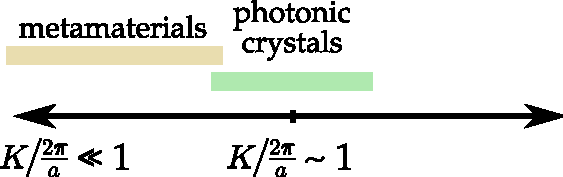
\includegraphics[width=8cm]{img/mm-phc-diagram.pdf} \end{figure} 

%%% XXX ============================== 1st band
Starting from the lowest frequencies, most periodic structures allow the Bloch wave to propagate. (An exception are conductive structures, see Chapter \ref{chap_wiremedium}, )  Due to very long wavelength, they can be easily treated as homogeneous medium and are usually classified as metamaterials operating in their first photonic band \cite{richter1995, kadlec2008, sibik2010dp}.
% in the author's view, this subset of metamaterials can be directly associated with the term of \textit{artificial dielectrics}

As far as the frequency of operation does not approach the upper edge of the first photonic band, these structures are completely nonresonant.  Let us stress that this classification is inseparably linked with specifying the frequency band of operation, since for any periodic structure, some electromagnetic resonances can be found at their respective frequencies.
The desired properties of nonresonant structures are obtained by averaging the properties of the constituent materials \cite{oganisian2014observation} or by engineering the unit cell are typically a strongly anisotropic tensor of permittivity \cite{kadlec2008, sibik2010dp}. Strictly speaking, this class of structures does not require periodicity, 

%%% XXX ============================== 1st band-gap
%%% XXX ============================== 2nd band
%%% XXX ============================== higher band-gaps and bands
\add{The notion of "wavelength", or more precisely "Bloch wavelength", is not uniquenly defined in such structures! }

\add{
		Resonant metamaterials operate in the 2nd BZ. From the arguments given in the Results section and in Ref. \cite{dominec2014transition}, on the example of dielectric rod array, the author conjectures that no useful metamaterial properties will be obtained from designing a linear metamaterial to operate in the third or higher photonic band.

		The studies of periodic electromagnetic structures is generally divided into two classes: the \textit{photonic crystals} and \textit{metamaterials}. These types of structures are formally very similar, as they are composed of 2-D or 3-D periodic array of unit cells, and the qualitative difference can be found only after the interaction with an electromagnetic wave is known. 

		%The difference is in the way how the unit cell interacts with the electromagnetic field. 

		Both types of structures exhibit the most interesting behaviour at their frequencies of resonance, but the different types of resonances define the technology and materials used to build them. The resonances in PhC rely on wave scattering, which can be easily obtained with any ordinary low-permittivity material such as silica or silicon. On the other hand, the resonances 
		%but the mentioned difference has profound consequences on the behaviour of the structure. 
		%}}}

		note \cite{silveirinha2007metamaterial}
		resonant metamaterials operate in the 2nd BZ (or possibly even third or higher? )
		Think over, note our paper dominec2014transition \cite{dominec2014transition}
}
\paragraph{Difference in the energy localisation}%{{{
... and resistance of the behaviour to the disorder

\add{Energy is the most localized at the frequencies of resonances.}

\mdf{In the photonic crystal (PhC), at its frequency range of operation, the effective wavelength is similar to the cell spacing and the cells scatter the propagating wave.
The energy of the resonant field is spread relatively evenly over the majority of the unit cell volume, which results in great sensitivity of the PhC behaviour to its periodicity and typically also in a high spatial dispersion. The most prominent phenomenon observed in PhC is the emergence of forbidden photonic bands around resonant frequencies, where the light can not propagate through the structure. 

On the contrary, the cells of a metamaterial (MM) are expected to exhibit individual resonances which should not significantly couple to each other. 
At the resonant frequencies in the metamaterials, the majority of the energy of the electromagnetic field is localised in a fraction of the unit cell volume, so that the behaviour of the metamaterial usually has only weak spatial dispersion, if any. This allows one to describe many metamaterials with acceptable precision as a homogeneous medium with a index of refraction $N(f)$, wave impedance $Z(f)$ and related effective permittivity $\varepsilon(f)=N/Z$ and permeability $\mu(f)=NZ$. 
}

\todo{If so, would be MMs a very narrow, or very broad  group of structures?}
%}}}
\paragraph{Difference in purpose and way of thinking}%{{{

The \textit{For Beginners} page of the ECONAM project states
Metamaterial is an arrangement of artificial structural elements, designed to achieve advantageous and unusual electromagnetic properties

existence of effective parameters

\cite{sihvola2009metamaterials}

\add{MMs are about HOW the light propagates. PhCs are about WHETHER the light propagates.}

%}}}

\subsection{Metamaterial homogenization} % note that NRW and CDH are discussed later
\paragraph{todo}%{{{
%% This is my approach only to a very complex problem; I can not solve all humankind's problems
Homogenization is not a search for an existing truth, but rather a somewhat arbitrary decision.

Effective parameters

ref Homogenisation issues - response to our paper from OpEx
\cite{rockstuhl2008transition}
\cite{paul2011reflection}
\cite{andryieuski2012bloch}
\cite{andryieuski2010homogenization} 
\cite{simovski2007bloch}
\cite{simovski2009material}
\cite{simovski2011electromagnetic}
\cite{mortensen2010unambiguous}
% todo{Elaborate mathematical treatise on this topic: \cite{sjoberg2005floquet}}
% A Floquet-Bloch decomposition of Maxwell's equations, applied to homogenization " The behavior of the solutions of a PDE with rapidly oscil-
%   lating coefficients, considered over distances large compared to the oscillations, is in several respects similar to the solutions of a PDE with slowly varying coefficients.
%   The problem of homogenization is to find these slowly varying coefficients by an ap- propriate limit process of the rapidly oscillating ones"

%% todo "process of replacing a complex structure of subwavelength sized components with an “effective medium” with uni-
%% form properties. It is a fundamentally important notion which can be traced back to the earliest days of electro-
%% magnetic theory, to the Lorentz-Lorenz and Maxwell-Garnet effective medium models [1–3]
%			[1] J. C. M. Garnett, Phil Trans. R. Soc. A 203, 385 (1904).
%			[2] D. E. Aspnes, Thin Solid Films 89, 249 (1982).
%			[3] W. Cai and V. Shalaev, Optical Metamaterials: Fundamentals and Applications (Springer, New York, 2010).

%% Many MMs do not bring negative refraction, other (composites) do, but not by means of resonances: 
%% The tunable negative permittivity and negative permeability of percolative Fe/Al2O3 composites in radio frequency range with
%% Negative index may arise from resonances

%}}}
\paragraph{"Negative-refraction", "negative-index", "left-handed" or "doubly-negative" media?}  %{{{
Media with a negative index of refraction are a subset of negative refraction, where the notion of index of refraction makes sense, as discussed above.

\add{When the index of refraction $N = \sqrt{\epsrl\murl}$ and the impedance $Z = \sqrt{\frac{\murl}{\epsrl}}$ are both defined, one may easily deduce that 
\begin{equation} \epsrl = \pm\frac{N}{Z}, \quad \murl = \pm N\,Z. \label{eq_nzepsmu}\end{equation}
The question of indefinite sign can be decided using the assumption of medium \textit{passivity}, that is, of the medium absorbing the wave rather than amplifying it. \todo{describe further}


\todo{add the comments from http://www.wave-scattering.com/negative.html}
}
%}}}

%% finish this? or leave this out?
%%      \section{Materials available for metamaterial construction}
%%      \subsection{General notes}
%%       complete it in the rest of the document!!
%%      \subsection{Dielectrics}
%%      \subsection{Metals}
%%      % and oxides for optical: Naik2011.pdf
%%      \subsection{Superconductors}
%%      \subsection{Tunable and switchable materials}
%%      \subsection{Specifics of the terahertz range}

%putting two resonances near to each other annihilates their “wings”
%→ hard to make a broadband-operating passive MM
%Metal eps spectra
%different models: Drude, lossy Drude
%spatial view of E+M wave propagation  (propagating/standing wave)
%in free space
%in arbitrary electromagnetic material 
%reflection on metal surface (PEC) and on PMC
%surface plasmons, standing/propagating
%non-lossy and lossy metal (-> quasi-bound states)
%Capacitive, inductive, resistive coupling?
%a “fast” and a “slow” resonance superposed?
%Two oscillators with nearly the same frequency:
%electric+electric or magnetic+magnetic → strong coupling, leads to twice curled curve in polar plot
%electric+magnetic → weak or no coupling (magnetic dipole: H field even, Efield odd; electric dipole: H field odd, E field even → may be regarded as zero inner product of the field functions)
%interpreting resonance (and Fano-resonance) curves
	%wave in free space → s12 ampli constant, phase constantly growing; (s11 zero)
	%→  in polar plot: a clockwise rotating unit vector
	%reflective surface → s11 ampli constant, phase constantly growing; (s12 zero)
	%simple resonance (in SRR?) 
	%→  reflectivity peak
	%→  losses
	%in polar plot of s12: fast clockwise curl, approaching zero point, phase up-DOWN-up
	%in polar plot of s11: clockwise curl starting at zero, making trip, returning to zero
	%Fano resonance: requires spiral segment of curve
	%case of "little fast curl 1" on "big slow curl 2"
	%if fres1 = fres2 → subtractive effect, both in amplitude and phase; phase up-down-UP-down-up
	%if fres1 < fres2 → …
	%find out the difference between:
	%two coupled broad resonances with interaction inbetween?

%Scaling and non-scaling properties [Zhou PRL 2005]
%(Mode curve anticrossing)
%Babinet principle
%(Quantum states in left-handed media?)
%
%Building metamaterials: key principles
%Homogenisation
%methods, issues, desired homogenized parameters
%Metal functions
%diluted metal → Pendry1996's low frequency plasmons
%metallic resonators: negative mu from SRR/Horseshoe/double-stripe
%Bianisotropy and chirality
%SRR and double-SRR
%keeping rotational-translational symmetry
%tunability
%MM impedance and coupling to free-space waves
%Mode coupling
%capacitive/resistive, behaviour, conditions, applications
%relations between MM and photonic crystal
%Higher-order Bloch modes
%
%Selected all-dielectric metamaterials
	%Mie resonances in high-permittivity microspheres
%
%Selected metalo-dielectric metamaterials
	%Aperture-array transmission
		%Wood anomaly in slit arrays
		%Wood anomaly in hole arrays
		%Standing SPP wave
	%“thin wires [8], [28], Swiss rolls [9], SRRs [9], electric SRRs (eSRRs) [29], [30], pairs of rods [10], [12], [31], pair of crosses [32], fishnets [17], [33]”
%
%== Weird ideas to elaborate ==
%* helical wire medium -> higher inductive load -> enables low plasma freq even for thicker wires
	%---> calculate FDTD
	%---> measure   TDTS with light bulb wires!
%* Possibility of standing phonon-polariton on SiC (!) 
%* try the anisotropic magnetic goo from the drawing board for children (but for electrical response)
%* find out how they could achieve negative phase speed
%* quantum point of view to negative phase/group velocity 

% TODO 2015-01-23: 
% 1) note that zero PBG width = dirac point = zero effective photon mass 
% 2) investigate how mode anticrossing relates to the significant spatial dispersion
% 3) find out why in effparam.py the data need to be conjugated, when MEEP seems to use the exp(-iwt) convention
% 4) possibly write into the numeric.tex about using the Debye model, with a scan for the damping coefficient (0.1 omega0 ... 100 omega0)
% 5) note about the meep peculiarity of notation: 'omega'=omega0/2pi , 'gamma'=gamma/2pi, 'sigma'=Deltaeps = F/omega0^2
